

\section{Minty mirth with options} 

Lego is a great toy. There are lots of little blocks, all different sizes and shapes, that snap together to form larger shapes. You can make caves and castles spaceships with the same set of blocks in new configurations. Options are a lot like lego. There are the basic blocks (vanilla \textbf{call} and \textbf{put} options) which can be combined to make combination strategies like \textbf{straddles}, and \textbf{strangles}, and \textbf{butterflies}. A little work and you can make \textbf{binaries}. Once you have binaries you can make almost anything. With enough binaries I can make a payoff diagram (profit on the x-axis, asset value on the y-axis) that spells out "MINTY MIrTH"  or "TWIrLY VYNYL"-- I'm completely serious. If you don't believe me I bet you a hundred dollars.  

With lego there are two types of children. One type follows the instruction manual precisely, perhaps counting out all the blocks first to ensure they correspond to the numbers on the box.  The other type might follow the instructions initially, but quickly innovates. The spaceship gets racing stripes and a dragon's tail. The country cottage gets rocket boosters, truck wheels, and a frightening amount of naval artillery. There are two corresponding types of option traders. One reads the rule book and creates neat standard structures with closed form pricing functions. The other type can make a dragon's tail out of butterfly wings. 

\section{Options and forwards again}

In the world of this chapter we have a single asset with price $S(t)$ at time $t$. We may buy the asset now at that price or a \textbf{claim} on the asset at time $T$ called the \textbf{expiry date}. There are three types of claims:

\begin{enumerate}
\item A \textbf{forward} which is the \textbf{obligation} to buy or sell the asset at a fixed price at $T$. The fixed price at time $t$ is $F_T(t)$. 
\item An \textbf{option} which is the \textbf{option} to buy or sell the asset at a fixed price at $T$. Call and put options to buy at price $K$ are denoted $C_{KT}$ and $P_{KT}$
\item A \textbf{zero coupon bond:} is a degenerate claim that pays \$1 no matter what happens. The bond is denoted $Z_T$
\end{enumerate}

The \textbf{value} of each of these contracts at time $t$ is denoted $V_{(.)}(t)$, so $V_{C_{KT}}(t)$ is the value at time $t$ of an option to buy the asset for $K$ at time $T$. 

At expiry time $T$ the contracts are valued:

\begin{itemize}
\item[] \textbf{Forward}: $V_{F}(T) = F_T(t)-S(T)$ \\
\item[] \textbf{Call option:} $V_{C_K}(T) = \max(S(T)-K,0)$\\
\item[] \textbf{Put option:} $V_{P_K}(T) =\max(K-S(T),0)$\\
\item[] \textbf{Bond:} $V_{Z_T}(T) = 1$
\end{itemize}

%The possibilities are depicted in figure \ref{fig:genericCPF}. These show the value of the contract at \textbf{expiry} as a function of the underlying price. Note that this is not the \textbf{profit} from holding these contracts because they have to be acquired at some price before expiry. 

Forwards, calls, and puts may be \textbf{bought} or \textbf{sold}. If a contract is bought it is sometimes called \textbf{long} and if sold \textbf{short}. So a \textbf{short put} is also a \textbf{sold put} denoted $-C_{K}$ with value at expiry $V_{-C_K}(T) = -\max(S(T)-K,0)$. 

Figure \ref{fig:genericCPFZ} has the expiry value  long and short forward, options, and bond. 

%A call option is an option to buy an asset (figure \ref{fig:genericCPF} (a)), a put option is an option to sell an asset (figure figure \ref{fig:genericCPF} (b)). A futures contract is an obligation to buy an asset (figure figure \ref{fig:genericCPF} ©). If you sell a call option or a put option or a future you get a mirror image of the payment (figures figure \ref{fig:genericCPF} (d), (e), and (f)). The figures give the \textbf{payoff} to each security as a function of the price of the underlying asset at expiry $S(T)$.  Call and put options cost money so the \textbf{profit} from the security is the payoff less the price. 

 \begin{figure}[ht]
\centering
  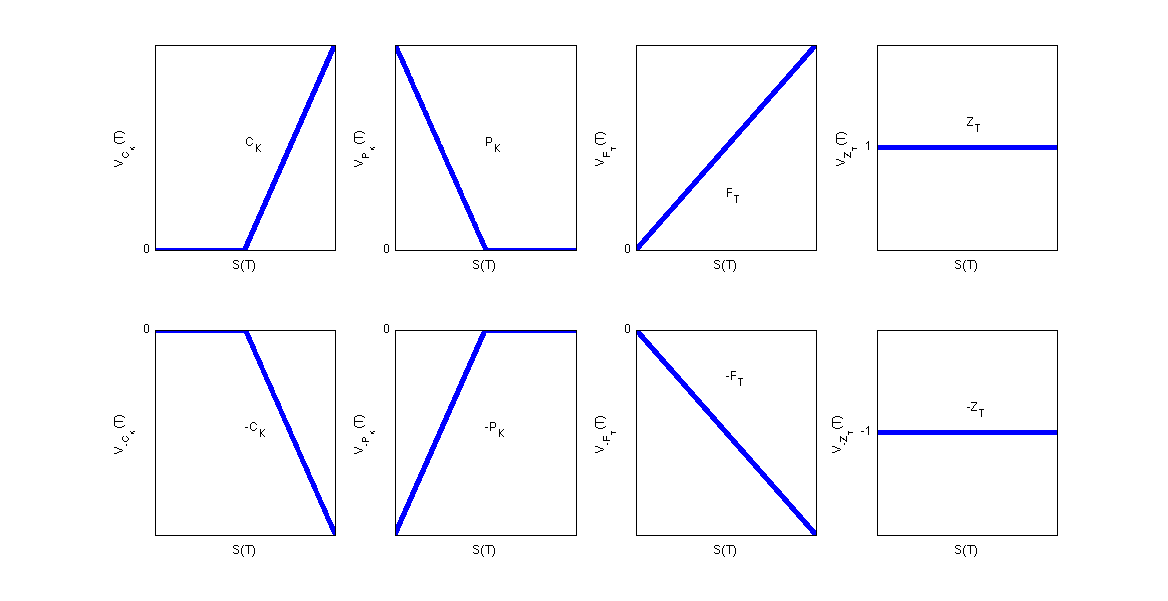
\includegraphics[width=5in] {pics/genericCPFZ}
\caption{Long and short call, put, and forward}
\label{fig:genericCPFZ}
\end{figure}

%To distinguish between a bought and sold option we'll prefix with "$+$" (bought) and "$-$" (sold). $V_{+C_{K,T}}(t)$ is the price of a bought call option with strike $K$ and expiry $T$ at time $t$. We won't bother subscripting the asset because we'll only deal with one asset in this chapter. 

%To be a little more confusing we'll sometimes identify the option by its sensitivity to the underlying asset (the \textbf{delta})\footnote{e.g. $delta(C_K) = \frac{\partial V_{C_K}}{\partial S(t)}$ rather than the strike. Write $C_{\mbox{delta}=x,T}$ for a call option with a delta equal to $x$.}

We'll use the following notation:

\begin{itemize}
\item $+ C_{K,T}$ bought call option with strike $K$ and expiry $T$
\item $+ C_{\mbox{delta}=x,T}$ bought call option with a delta of $x$ and expiry $T$
\item $+ C_{ATM}$ is the at-the-money option where strike is equal to current asset price.
\item $- P_{K,T}$ sold call option with strike $K$ and expiry $T$
\item $+F_T$ bought  futures contract with delivery at $T$ 
\item $F_T(t)$ the price of the futures contract at time $t$. 
\item $Z_T$ a zero coupon bond paying \$1 at time $T$.
\item $V_{+C_{K,T}}(T)$ value of call option at expiry
\item $\sigma_{K,T}$ is the implied volatility for calls and puts at strike $K$ and maturity $T$
\item $\sigma_{\mbox{delta}=x,T}$ is the implied volatility for calls with a delta of $x$. 
\item $r(T)$ is the risk free rate for a bond maturing at $T$.
\item $B^{x,y}_K$ is a \textbf{binary} which is worth $x$  (introduced later).
\end{itemize}

A few additional points to recall:

\begin{enumerate}
\item The \textbf{present value} at time $t$ of a claim on \$1 at time $T$ is the price of the bond $V_{Z_T}(t)$. 
\item The \textbf{future value} at time $T$ of a \$1 payment now is $\frac{1}{V_{Z_T}(t)}$
\item The \textbf{implied volatility} of an option is a parameter from the Black-Scholes-Merton pricing formula but this is only a convenience. Each implied volatility gives a unique price so an implied volatility quote is just another way of quoting price. We don't have to satisfy the Black-Scholes assumptions for this to be useful.
\item The \textbf{delta} of an option is the sensitivity of the option price to the underlying asset price. For each delta there is a unique strike so delta is just another way of quoting strike.
\end{enumerate}

These are the basic building blocks. From here we start building combinations.

\subsection{Making combinations}

We'll add together quantities of calls, puts, forwards, and bonds to make \textbf{structures}. Two examples illustrate simple structures:

\textbf{Example: $+C_{K,T}-P_{K,T}$}\\
Buy a call option and sell a put option at the same strike. The combined payoff is a straight line (see figure \ref{fig:CmP}) How interesting. 
 
 \begin{center}
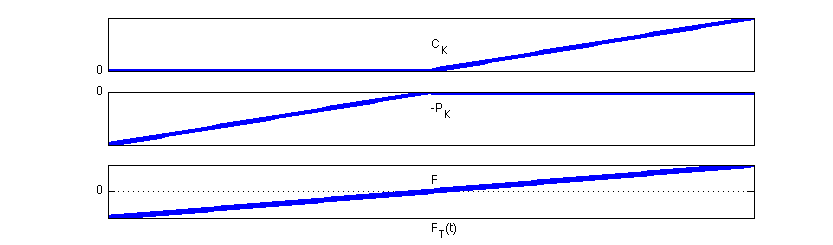
\includegraphics[width=5in]{pics/CmP}%
\captionof{figure}{Buy call, sell put}\label{fig:CmP}%
\end{center}
 
%  \begin{figure}[!htbp]
%\centering
 % 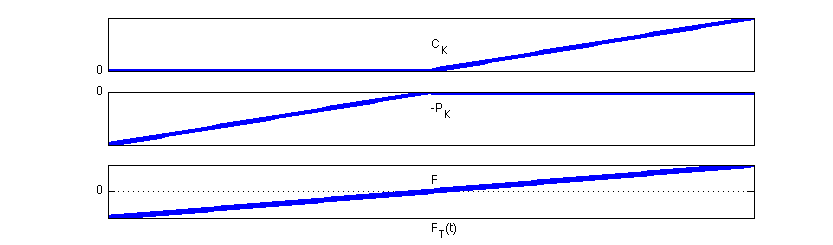
\includegraphics[width=5in] {pics/CmP}
%\caption{Buy call, sell put}
%\label{fig:CmP}
%\end{figure}
 
 \textbf{Example: $+C_{K_1,T}-C_{K_2,T}$}\\
Buy a call option at strike $K_1$ and sell a call option at strike $K_2$. Up to $K_2$ the payoff is the same as $C_{K_1}$ but then the gains from the $C_{K_1}$ are offset by losses from the $C_{K_2}$ (figure \ref{fig:CK1mCK2_1})
 
  \begin{center}
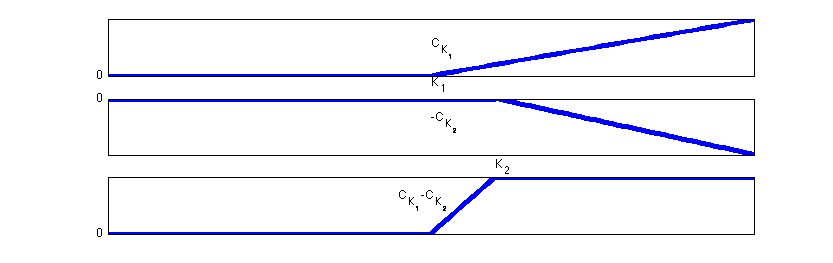
\includegraphics[width=5in]{pics/CK1mCK2}%
\captionof{figure}{Buy call at $K_1$, sell call at $K_2$}\label{fig:CK1mCK2_1}%
\end{center}
 
%  \begin{figure}[!htbp]
%\centering
 % 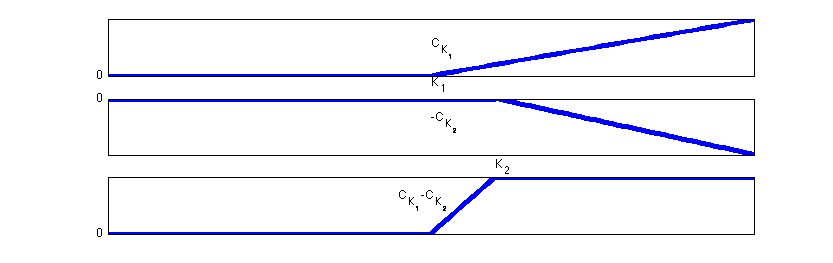
\includegraphics[width=5in] {pics/CK1mCK2}
%\caption{Buy call at $K_1$, sell call at $K_2$}
%\label{fig:CK1mCK2}
%\end{figure}
 
We could add many options, futures, and bonds together in a similar way. 

\subsection{Put call parity}

In the first example above the combined $+C_K-P_K$ makes a straight line. If we add in a $-F$ we get a horizontal line equal to $F_T(t)-K$ (figure \ref{fig:CmPmF}). 

  \begin{center}
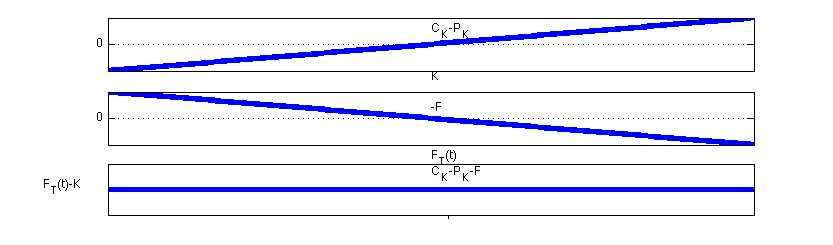
\includegraphics[width=5in]{pics/CmPmF}%
\captionof{figure}{Buy call at $K$, sell call at $K$, sell forward}\label{fig:CmPmF}%
\end{center}

%  \begin{figure}[ht]
%\centering
 % 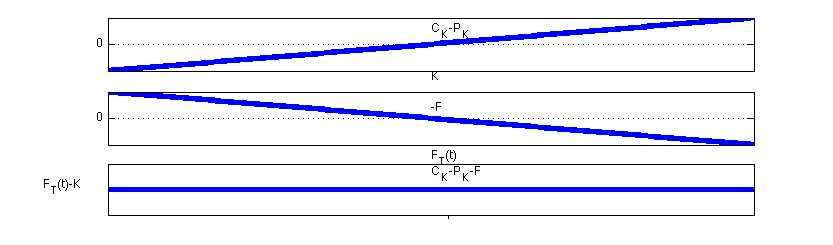
\includegraphics[width=5in] {pics/CmPmF}
%\caption{Buy call at $K$, sell call at $K$, sell forward}
%\label{fig:CmPmF}
%\end{figure}

So if we buy a call, sell a put, and buy a forward, we have a guaranteed payoff of $F_T(t)-K$ no matter what happens. A guaranteed payment can be priced with the risk free bond, so \$1 at time $T$ is worth $Z_T(T)$ now: 

\[V_{-P_{K,T}}(t)+ V_{+C_{K,T}}(t)  = (F_T(t)-K) V_{Z_T}(t) \]

This must be true at all times otherwise there would be an arbitrage. If the options are struck at the forward price ($K= F_T(t)$) then the combination must be worth zero (figure \ref{fig:CmPmF0})

\[K=F_T(t) \Rightarrow V_{-P_{K,T}}(t)+ V_{+C_{K,T}}(t) = 0 \]

  \begin{center}
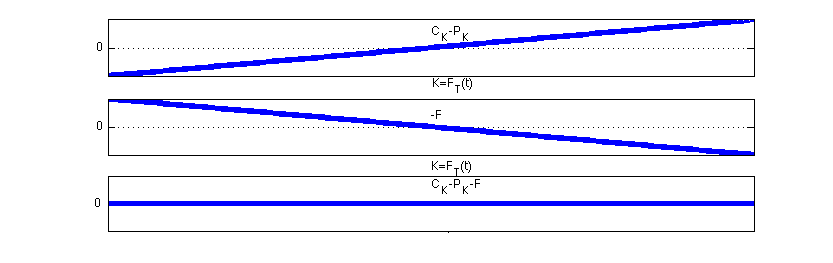
\includegraphics[width=5in]{pics/CmPmF0}%
\captionof{figure}{Buy call at $K - F_T(t)$, sell call at $K = F_T(t)$, sell forward}\label{fig:CmPmF0}%
\end{center}

%  \begin{figure}[ht]
%\centering
 % 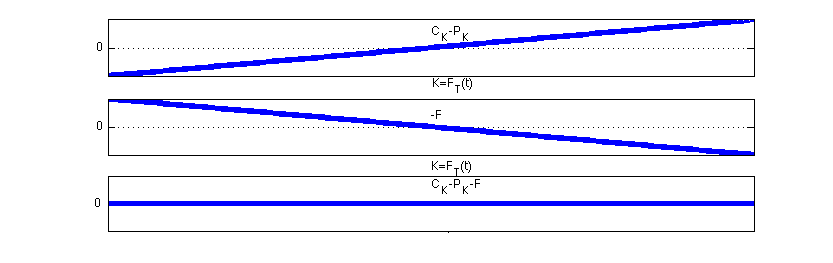
\includegraphics[width=5in] {pics/CmPmF0}
%\caption{Buy call at $K - F_T(t)$, sell call at $K = F_T(t)$, sell forward}
%\label{fig:CmPmF0}
%\end{figure}


So the call and the put have the same price. This relationship is called \textbf{put call parity}. It's very powerful because it allows us to substitute puts for calls. With a call option I can create a put option by selling a forward and buying $\frac{(F_T(t)-K)}{V_{Z_T}(t)}$ of the zero coupon bond. When the bond matures it will be worth $(F_T(t)-K)$ and the circle of life will be complete. If the options have a strike equal to the forward price I only have to sell the forward to create the put. If we like we can forget about puts altogether. 

%A couple of implications of put call parity are:

%\begin{itemize}
%\item The delta of a call minus 1 is the delta of a put at the same strike. 
%\item Call and put options at the same strike have the same \textbf{implied volatility}. Why? Why don't you tell me? 
%\end{itemize}

\section{Five easy combinations}

We'll build five basic option structures. They have funny names like \textbf{strangle}, \textbf{straddle}, and \textbf{butterfly}. Traders like to give things funny names because it makes them feel like they're part of a special club with a secret language. 

%There's a secret handshake too but I'm not allowed to tell you about that.

\subsection{Straddle}

\begin{center}
\begin{tabular}{|cc|}
\hline
\textbf{Ingredients:} & $+C_{K} +P_{K}$\\
\textbf{Looks like:}  &The letter "V" (figure \ref{fig:CpP})\\
\textbf{Characteristics:} & \parbox{3in}{Limited loss, unlimited gain. Makes money if the market moves too much in either direction. Loses money if the price doesn't change too much.}\\
\hline
\end{tabular}
\end{center}

 \begin{figure}[ht]
\centering
  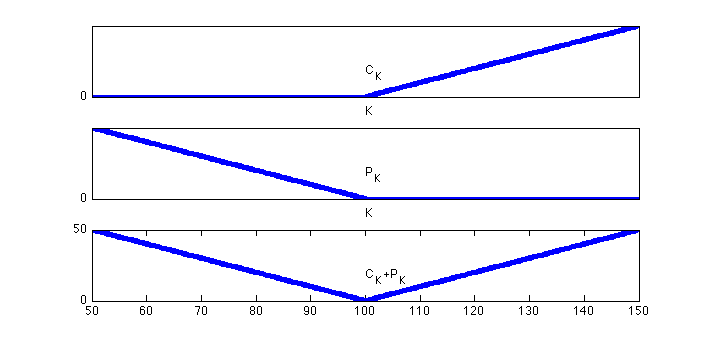
\includegraphics[width=5in] {pics/CpP}
\caption{Straddle: buy call at $K$, buy put at $K$}
\label{fig:CpP}
\end{figure}


\subsection{Strangle}

\begin{center}
\begin{tabular}{|cc|}
\hline
\textbf{Ingredients:} & $+C_{K_2} +P_{K_1}$, $K_1<K_2$\\
\textbf{Looks like:}  & A badly drawn boat (figure \ref{fig:CK2pPK1})\\
\textbf{Characteristics:} & \parbox{3in}{Limited loss, unlimited gain. Makes money with extreme market moves in either direction. Cheaper than a straddle because both options are are out of the money.}\\
\hline
\end{tabular}
\end{center}


  \begin{figure}[ht]
\centering
  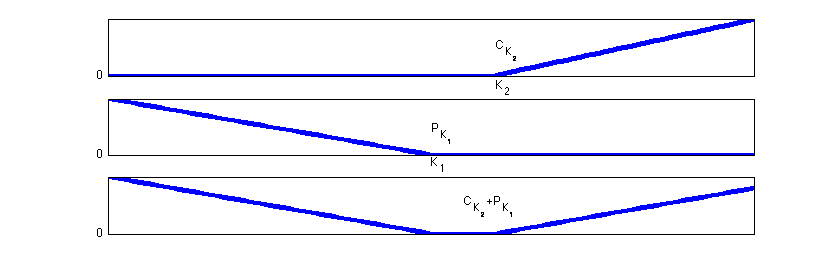
\includegraphics[width=5in] {pics/CK2pPK1}
\caption{Strangle: buy call at $K_2$, buy put at $K_1$}
\label{fig:CK2pPK1}
\end{figure}

\subsection{Collar}

\begin{center}
\begin{tabular}{|cc|}
\hline
\textbf{Ingredients:} &$+C_{K_1} -C_{K_2}$, $K_1>K_2$\\
\textbf{Looks like:}  & Nothing like a collar. More like a ramp. (figure \ref{fig:CK1mCK2})\\
\textbf{Characteristics:} & \parbox{3in}{Limited loss, limited gain. A little bit like a long position except nothing
happens if the price is between $K_1$ and $K_2$ at expiry.}\\
\hline
\end{tabular}
\end{center}

  \begin{figure}[ht]
\centering
  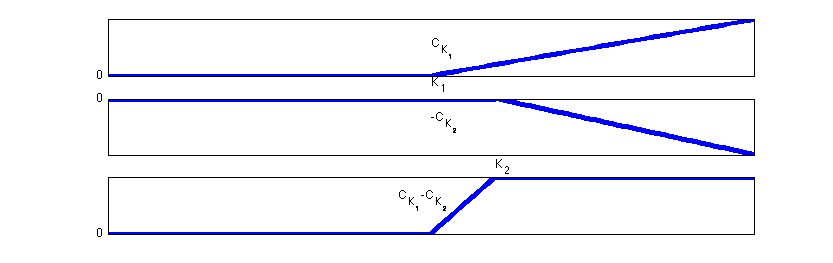
\includegraphics[width=5in] {pics/CK1mCK2}
\caption{Collar: buy call at $K_1$, sell call at $K_2$}
\label{fig:CK1mCK2}
\end{figure}

\subsection{Risk reversal}

\begin{center}
\begin{tabular}{|cc|}
\hline
\textbf{Ingredients:} &$+P_{K_1}  - C_{K_2}$\\
\textbf{Looks like:}  & Nothing really (figure \ref{fig:PK1mCK2})\\
\textbf{Characteristics:} & \parbox{3in}{Limited gain, unlimited loss. Makes money if the market goes down a lot, loses money if the market goes up a lot, otherwise does nothing.}\\
\hline
\end{tabular}
\end{center}


 \begin{figure}[ht]
\centering
  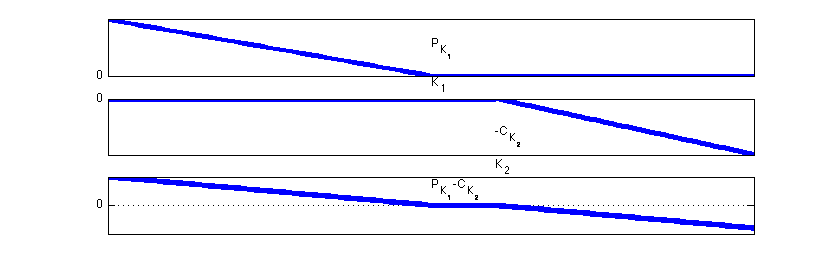
\includegraphics[width=5in] {pics/PK1mCK2}
\caption{Risk reversal: buy put at $K_1$, sell call at $K_2$}
\label{fig:PK1mCK2}
\end{figure}


\textbf{Delta quoted risk reversals}\\
Risk reversals are also often quoted in terms of implied volatility at a fixed delta. A 10-delta risk reversal has a 10 delta call and a 10 delta put:

\[RR_{\mbox{delta} = 10}= -P_{\mbox{delta}=10} + C_{\mbox{delta}=10}\]

%When this is quoted in terms of implied volatility it gives a measure of \textbf{volatility skew} in the implied volatility curve. If the risk reversal is quoted as positive it means the implied volatility is higher for the higher strike.

Risk reversals are often quoted in volatility points. For example a 25 delta risk reversal is the 25 delta put (75 delta call) minus the 25 delta call. The risk reversal is quoted as the difference between these two implied volatilities:

\[ \sigma_{\mbox{25 delta RR}} = \sigma_{\mbox{delta} = 75} - \sigma_{\mbox{delta} = 25}    \]

\subsection{Butterfly}


\begin{center}
\begin{tabular}{|cc|}
\hline
\textbf{Ingredients:} &$+C_{K_1} -2*C_{K_2} + C_{K_3}$\\
\textbf{Looks like:}  &A tent (figure \ref{fig:CK1m2CK2pCK3})\\
\textbf{Characteristics:} & \parbox{3in}{Limited loss, limited gain. Makes money if market doesn't move too far in either direction.}\\
\hline
\end{tabular}
\end{center}

 \begin{figure}[ht]
\centering
  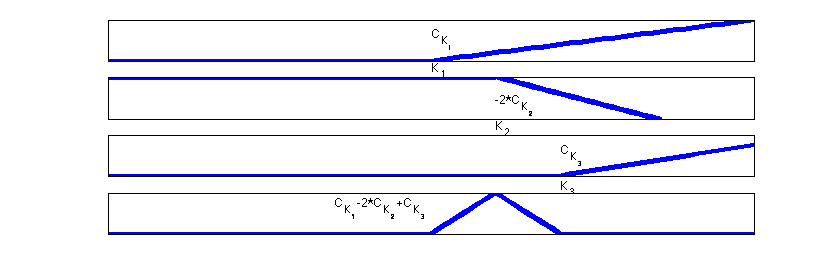
\includegraphics[width=5in] {pics/CK1m2CK2pCK3}
\caption{Butterfly: buy call at $K_1$, sell two calls at $K_2$, buy call at $K_3$}
\label{fig:CK1m2CK2pCK3}
\end{figure}

\textbf{Delta quoted butterflies}\\
Butterflies are also often quoted in terms of \textbf{delta}. A 25-delta butterfly is 

\[BF_{\mbox{delta} = 25} = +C_{\mbox{delta}=75} -2*C_{\mbox{delta}=50} + C_{\mbox{delta}=25}\]

 In this convention the middle option is at 50-delta. This is a good convention because it makes the whole structure \textbf{delta neutral}:

\[\mbox{delta}(\mbox{25 delta BF})= \mbox{delta}(C_{\mbox{delta}=75}) -2*\mbox{delta}(C_{\mbox{delta}=50})+ \mbox{delta}(C_{\mbox{delta}=25}) = 0\]  


If the butterfly is quoted in volatility points it gives a measure of \textbf{kurtosis}. If the butterfly is quoted as positive it means the average implied volatility of the 75 and 25 delta options is bigger than the 50-delta implied volatility.

\[ \sigma_{\mbox{25 delta BF}}  = \sigma_{\mbox{delta} =75} - 2*\sigma_{\mbox{delta}=50} + \sigma_{\mbox{delta} = 25} \]

The next section gives an example.
 

\section{A convenient quotation convention in three numbers}

If we quote the risk reversal and butterfly in implied volatility and with delta we can use a neat quotation convention using the 50 delta option and a butterfly and risk reversal at the same delta. For example we might have

\begin{itemize}
\item Implied volatility of 50 delta option is 0.2
\item 25-delta butterfly is 0.05
\item 25-delta risk reversal is -0.02
\end{itemize}

We can determine that:

\begin{itemize}
\item[(a)] Since the butterfly implied volatility is positive the out of the money options have higher average implied volatility than the 50 delta (there is a \textbf{volatility smile}), and\\
\item[(b)] Since the risk reversal implied volatility is negative the higher strike has a lower implied volatility than the lower strike (the volatility curve is \textbf{positively skewed}, so the smile is a \textbf{smirk}).
\end{itemize}

We can also figure out the implied volatility at three points in the volatility curve. We have 

\[\sigma_{\mbox{25 delta RR}} = -\sigma_{\mbox{delta}=75} +\sigma_{\mbox{delta}=25} = -0.02 \]

\[\sigma_{\mbox{25 delta BF}} = \sigma_{\mbox{delta}=75} -2*\sigma_{\mbox{delta}=50}+ \sigma_{\mbox{delta}=25} = 0.05 \]

Rearrange and substitute in for the 50 delta implied and we have 

\[\sigma_{\mbox{delta}=25} = 0.215\]

 and 
 
 \[ \sigma_{\mbox{delta = 75}} = 0.235 \]
 
Part of the volatility curve might look like figure \ref{fig:volcurveEg}.

  \begin{center}
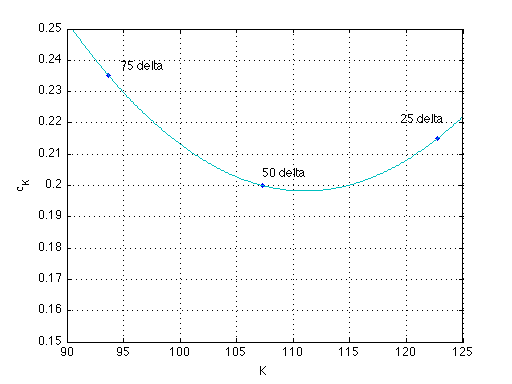
\includegraphics[width=5in]{pics/volcurveEg}%
\captionof{figure}{Volatility curve}\label{fig:volcurveEg}%
\end{center}

% \begin{figure}[ht]
%\centering
 % 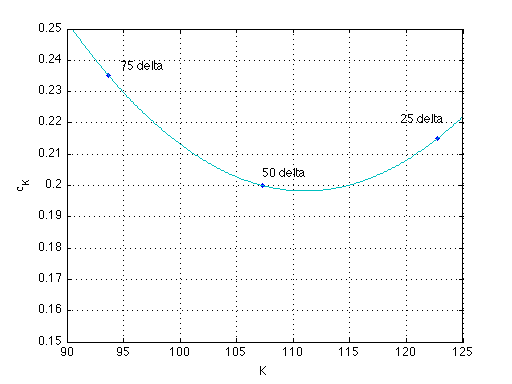
\includegraphics[width=5in] {pics/volcurveEg}
%\caption{Volatility curve}
%\label{fig:volcurveEg}
%\end{figure}




\section{Greek hedging}

The value of options and option portfolios have four important determinants of which the sensitivities are the \textbf{greeks}:

\begin{center}
\begin{tabular}{|c|c|}
\hline
Sensitivity & Greek \\
\hline
\textbf{Current asset price} $S(t)$ & $\mbox{delta} = \frac{\partial V}{\partial S}$\\
\textbf{Delta} & $\mbox{gamma} = \frac{\partial \mbox{delta}}{\partial \mbox{S}} = \frac{\partial V}{(\partial S)^2}$\\
\textbf{Implied volatility} (at some strike and expiry) $\sigma_{KT}$ & $\mbox{vega} = \frac{\partial V}{\partial \sigma_{KT}}$\\
\textbf{Interest rates} (at some maturities) $r(T)$ & $\mbox{rho} = \frac{\partial V}{\partial r(T)}$\\
\textbf{Time to expiry} $T-t$ & $\mbox{theta} = -\frac{\partial V}{\partial t}$\\
\hline
\end{tabular}
\end{center}

The idea of \textbf{greek hedging} is that the sensitivity of a portfolio to these things can be offset selectively by holding a \textbf{hedging portfolio} which has the negative value of the target greek. 

Figure \ref{fig:greekTangents} has the time $t$ value of a call option exporting at $T$ as a function of asset price, implied volatility, the interest rate, and time to expiry. The first order sensitivity is the value of the tangent line to the function. For an example we'll use an option with $K = S(t) = 100$, $r(T) = 0.05$, $T-t = 1$, and $\sigma_{100,1} = 0.2$. 

  \begin{center}
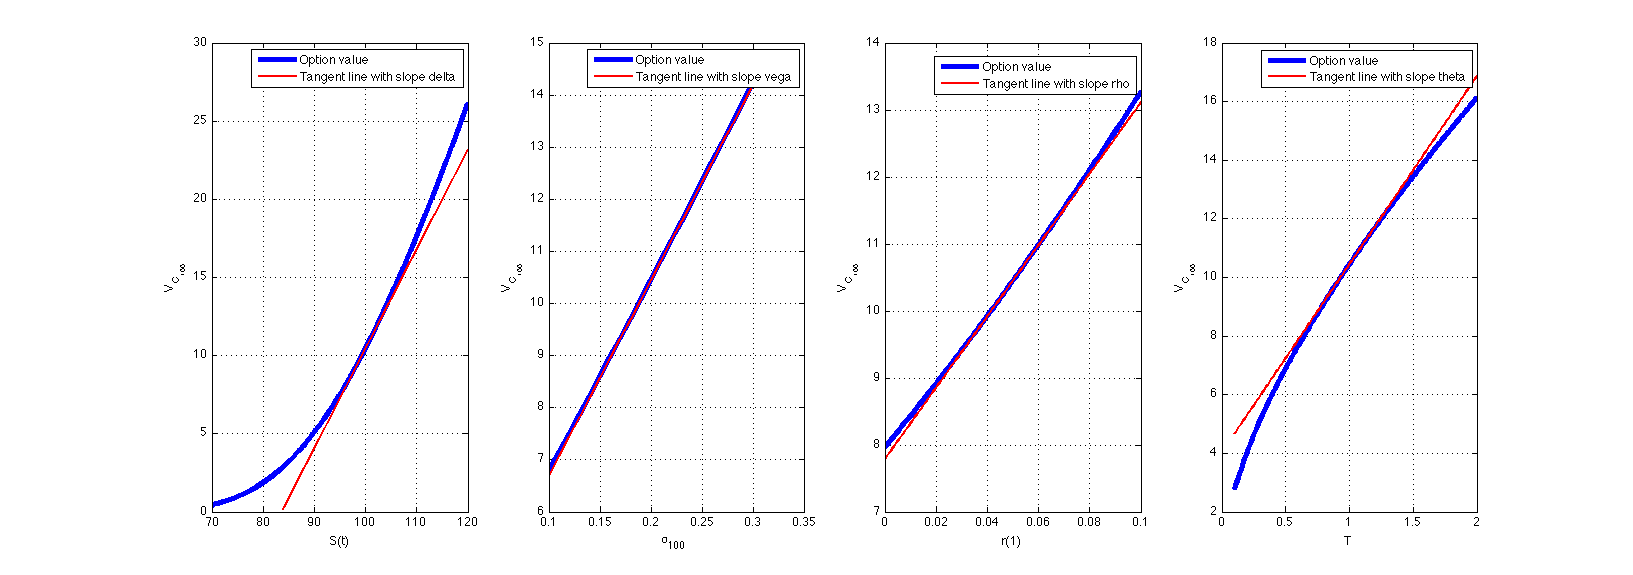
\includegraphics[width=5in]{pics/greekTangents}%
\captionof{figure}{Option sensitivities}\label{fig:greekTangents}%
\end{center}

% \begin{figure}[ht]
%\centering
 % 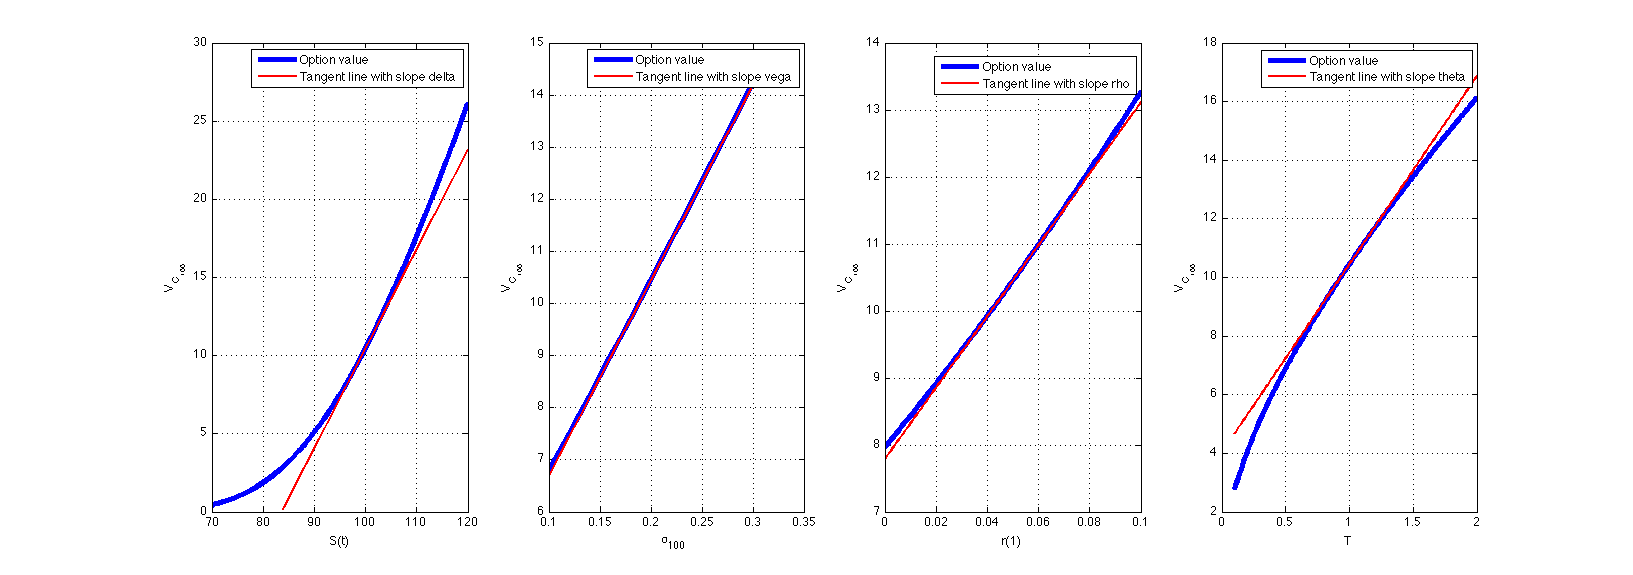
\includegraphics[width=5in] {pics/greekTangents}
%\caption{Option sensitivities}
%\label{fig:greekTangents}
%\end{figure}

To hedge the greeks is to create a hedge portfolio mirroring the tangent line in each picture. In the examples we'll use two options (100 strike call and 70 strike call), the underlying asset, and a zero coupon bond: 

\begin{center}
\begin{tabular}{|c|cccc|}
\hline
 & delta & gamma & vega & rho\\
\hline
$C_{100}$ & 0.64 & 0.19 & 37.52 & 53.23\\
$C_{70}$ & 0.98 & 0.02 & 4.10 & 64.82\\
$S$ & 1  & 0 & 0 & 0\\ 
$Z_1$ & 0 & 0 & 0 & -95.12\\
\hline
\end{tabular}
\end{center}

\subsection{An almost general form for portfolio sensitivities}

The change in the value of a portfolio is $\Delta V$ can be decomposed to a function of changes in underlying, interest rate, implied volatility, and time.

\begin{eqnarray*}
dV &\approx \frac{\partial V}{\partial S} \Delta S + 0.5\frac{\partial^2V}{(\partial S)^2}(\Delta S)^2 + \left( \sum_K \sum_T \frac{\partial V}{\partial \sigma_{KT}} \Delta \sigma_{KT}  \right) + \sum_T \frac{\partial V}{\partial r_T} \Delta r_T + \frac{\partial V}{\partial t} \Delta t\\
 &= \mbox{delta}\Delta S + 0.5\mbox{gamma}(\Delta S)^2 +  \left( \sum_K \sum_T \mbox{vega}\Delta \sigma_{KT} \right) \sum_T \mbox{rho} \Delta r_T + \mbox{theta} \Delta t\\
\end{eqnarray*}

This uses the two term Taylor series for price and one term for everything else. For more precision we can include more terms in the series. A greek hedge to a factor $x$ is an asset with value $H$ that offsets the exposure:

\begin{eqnarray*}
\frac{\partial H}{\partial x} = -\frac{\partial V}{\partial x}\\
\Rightarrow \frac{\partial (H + V)}{\partial x} = 0
\end{eqnarray*}

\subsection{Delta hedging}

A delta hedge needs an exposure to the underlying asset. We could use the asset itself, a \textbf{futures contract}, or another option. Using an option to hedge delta is not usually a good idea because the new option will add new sensitivities to volatility, rates, and time. Delta hedges usually use the underlying asset or the forward because they don't much disturb the rest of the option value eco-system. 

Figure \ref{fig:deltaHedge} illustrates a delta hedge of the $C_{100}$ option with a short position in the underlying asset. The first panel is the call option value against the underlying price ($S(t) = 100$, $K = 100$, $r = 0.05$, $T-t=1$).  The second panel is a short position in the asset holding -0.638 units (the delta). The third panel is the combined portfolio. The delta hedge removes the sensitivity to the asset. At $S(t)=100$ the sensitivity is zero. 

As the price changes the hedge must be changed. A delta hedge must be adjusted periodically to keep this sensitivity close to zero.

%If the hedge is maintained to expiry,  and under some strict conditions\footnote{The price is determined by Geometric Brownian Motion with a constant volatility and the hedge is adjusted continuously}, the discounted value of the combined portfolio will be zero when the option expires. 

\begin{center}
\begin{tabular}{|c|cc|}
\hline
 & Name & delta\\
\hline
Option & $C_{100}$ & 0.68\\
Hedge & $S$ & 1\\
\hline
\end{tabular}
\end{center}

\begin{eqnarray*}
\mbox{delta}(C_{100}) = 0.638\\
\mbox{delta}(-0.638*S) = -0.638\\
\mbox{delta}(C_{100} -0.638*S) = 0
\end{eqnarray*}

Where $\mbox{delta}(.)$ is the combined delta.

  \begin{center}
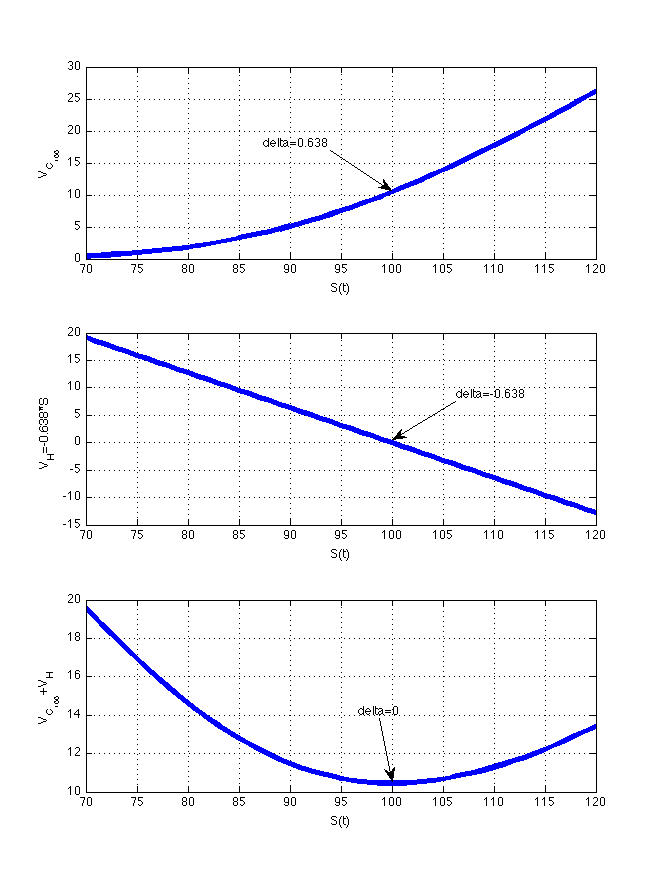
\includegraphics[width=4in]{pics/deltaHedge}%
\captionof{figure}{Delta hedge}\label{fig:deltaHedge}%
\end{center}

% \begin{figure}[ht]
%\centering
 % 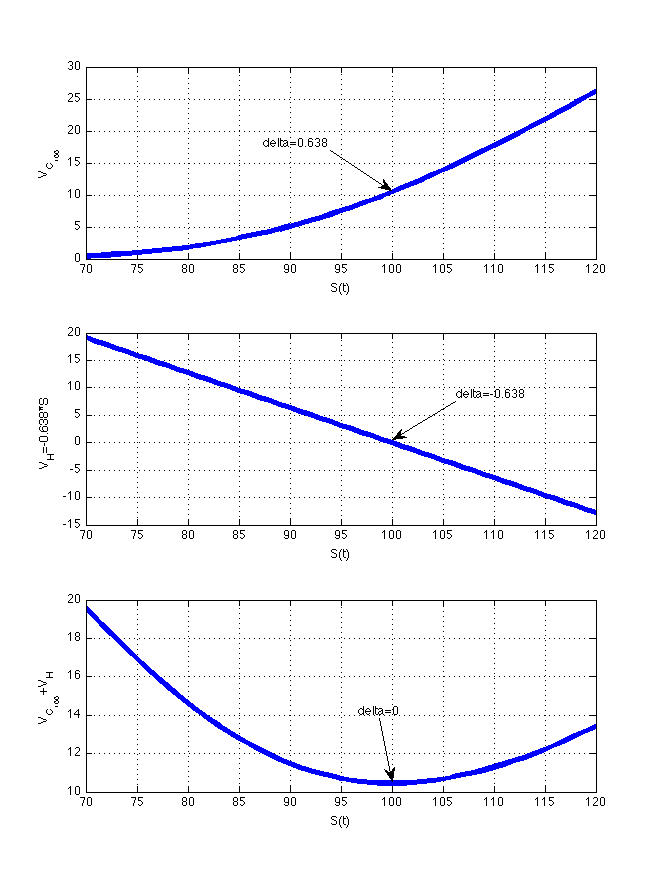
\includegraphics[width=5in] {pics/deltaHedge}
%\caption{Delta hedge}
%\label{fig:deltaHedge}
%\end{figure}

\subsection{Gamma hedging}

Gamma hedging is a bit stranger. With gamma hedging we're hedging the \textbf{curvature} of the option payoff against the strike. We can't do this with futures or the underlying asset because they're both linear. We need a \textbf{non-linear} payoff. The most ready source of curvature is other options.  

Say we have another option, a call struck at 70 with a gamma of 0.002. This option has a positive gamma so selling it gives a negative gamma. The call at 100 has a gamma of 0.019 so we need -9.16 of the 70 strike options to hedge the gamma. Figure \ref{fig:gammaHedge} gives the story. The first panel is our original option; the second panel is -9.16 of the $C_{70}$ options; the third panel is the combined portfolio.


\begin{center}
\begin{tabular}{|c|cc|}
\hline
 & Name & gamma\\
\hline
Option & $C_{100}$ & 0.019\\
Hedge & $C_{70}$ & 0.02\\
\hline
\end{tabular}
\end{center}

\begin{eqnarray*}
\mbox{gamma}(C_{100}) = 0.19\\
\mbox{gamma}(C_{70}) = 0.02\\
\mbox{gamma}(-9.16*C_{70}) = -0.19\\
\mbox{gamma}(C_{70} + -9.16*C_{70}) = 0
\end{eqnarray*}

Where $\mbox{gamma}(.)$ is the combined gamma.

  \begin{center}
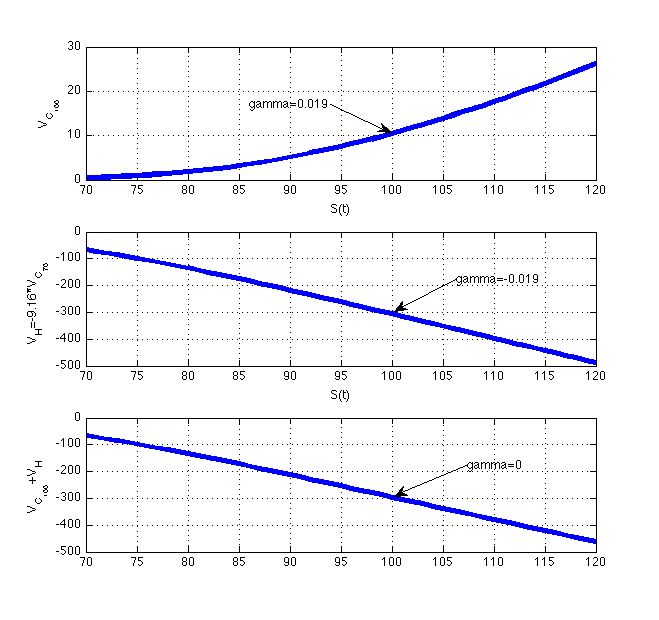
\includegraphics[width=3in]{pics/gammaHedge}%
\captionof{figure}{Gamma hedge}\label{fig:gammaHedge}%
\end{center}


% \begin{figure}[ht]
%\centering
 % 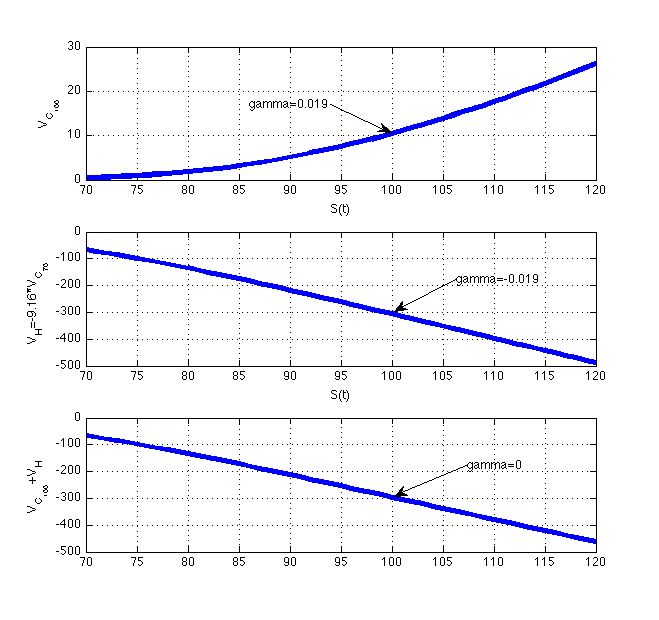
\includegraphics[width=5in] {pics/gammaHedge}
%\caption{Gamma hedge}
%\label{fig:gammaHedge}
%\end{figure}



\textbf{Delta-Gamma hedging}

The trouble with gamma hedging is that it introduces other sensitivities. A $C_{70}$ option brings $0.98$ deltas, $0.02$ gammas, 4.1 vegas, and 64.82 rhos.  We could go mad trying to plug up all those holes only to open others. A compromise is to only hedge out the additional delta. This is straightforward. We need -9.16 of the $C_{70}$'s to hedge the gamma which introduces $-0.98*9.16 = -9.01$ deltas. The original $C_{100}$ option has $0.64$ deltas so we need $9.01-0.64 = 8.37$ units of the asset for a delta hedge of the combination. 

The first panel of \ref{fig:deltaGammaHedge}  is the option, the second panel is -9.01 of the $C_{70}$ option for the gamma hedge, and the third panel is a delta hedge with 8.37 of the underlying . The result is in the fourth panel which I think you would agree cuts a much sleeker figure.  At $S(t)=100$ the total portfolio is delta and gamma neutral. Graphically the portfolio has zero slope \textit{and} zero curvature at $S(t)=100$, though both are nonzero away from this point.

\begin{center}
\begin{tabular}{|c|ccc|}
\hline
 & & delta & gamma\\
\hline
Option & $C_{100}$ & 0.64 & 0.19\\
Hedge & $C_{70}$ & 0.98 & 0.02\\
Hedge & $S$ & 1 & 0\\
\hline
\end{tabular}
\end{center}

\begin{eqnarray*}
\mbox{gamma}(C_{100}) = 0.19\\
\mbox{gamma}(C_{70}) = 0.02\\
\mbox{gamma}(-9.16*C_{70}) = -0.19\\
\mbox{gamma}(C_{100}-9.16*C_{70}) = 0
\end{eqnarray*}

\begin{eqnarray*}
\mbox{delta}(C_{100}) = 0.64\\
\mbox{delta}(C_{70}) = 0.98\\
\mbox{delta}(C_{100} -9.16*C_{70}) = -8.37\\
\mbox{delta}(8.37*S) = 8.37\\
\mbox{delta}(C_{100} -9.16*C_{70}+8.37*S) = 0
\end{eqnarray*}

  \begin{center}
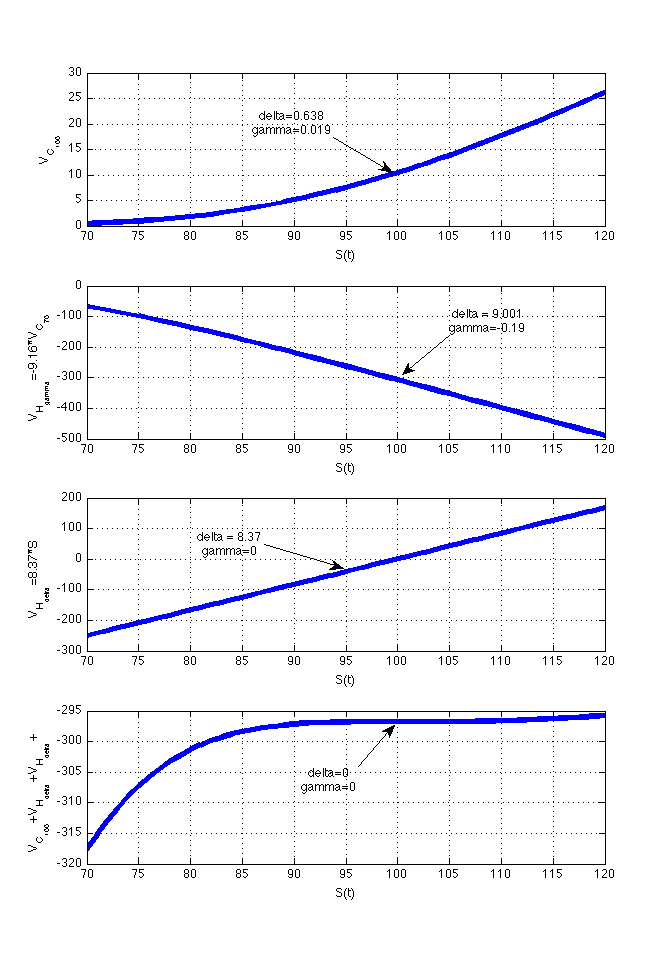
\includegraphics[width=3.5in]{pics/deltaGammaHedge}%
\captionof{figure}{Delta-gamma hedge}\label{fig:deltaGammaHedge}%
\end{center}

% \begin{figure}[ht]
%\centering
 % 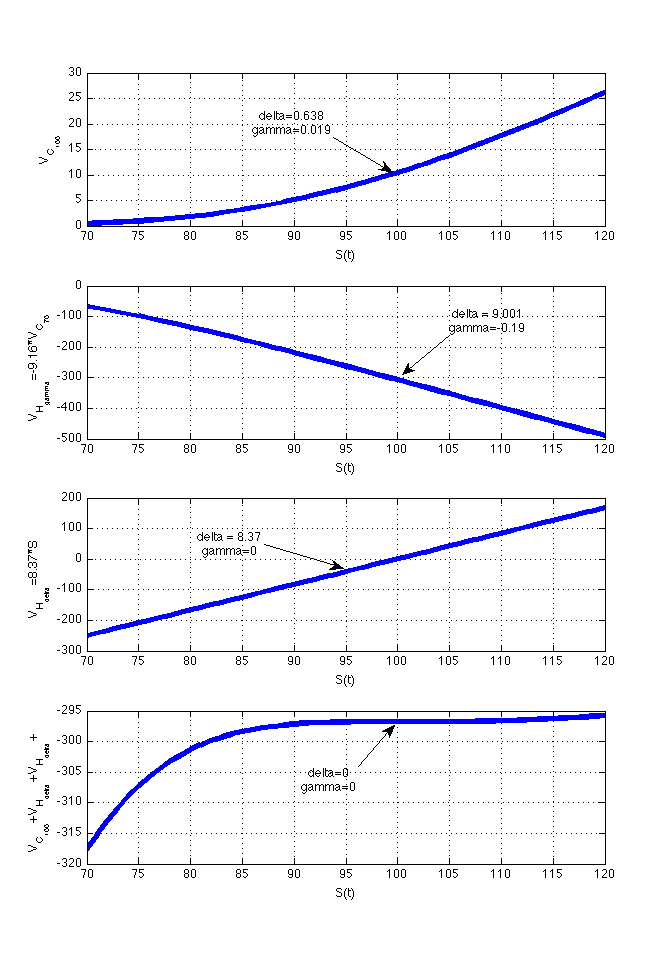
\includegraphics[width=4in] {pics/deltaGammaHedge}
%\caption{Delta-gamma hedge}
%\label{fig:deltaGammaHedge}
%\end{figure}

\subsection{Vega hedging}

Vega hedging is a similar process. Each option has an exposure to implied volatility $\sigma_{KT}$. We have to find another asset that also has an exposure to $\sigma_{KT}$. This is where the trouble starts. Unless you can find someone selling an asset with an exposure to $\sigma_{KT}$ that \textit{isn't} the original option you can't get a hedge. 

We can get around this by hedging with a different option and assuming that the volatility curve moves in parallel, i.e. 

\[ \Delta \sigma_{K_1} =  \Delta \sigma_{K_2} \forall K_1,K_2 \] 

This is only a slightly heroic assumption. Volatility moves fairly constantly across the curve. If the implied volatility at 100 increases by 0.01 the implied volatility at 70 will usually move by something similar. So you can hedge the vega of one option by holding another option. Sort of.

Fixed income nerds will note that a similar approach is taken with duration hedging in fixed income. Basic duration measures assume a parallel shift in rates across the yield curve, just as here we assume a parallel shift across the volatility curve. Some people like to model the joint behaviour of the volatility curve (and the yield curve). That's a more complicated exercise.

Assuming that the volatility curve always moves the same amount at each point:

\begin{center}
\begin{tabular}{|c|cc|}
\hline
 & & vega\\
\hline
Option & $C_{100}$ & 37.52\\
Hedge & $C_{70}$  & 4.1\\
\hline
\end{tabular}
\end{center}

\begin{eqnarray*}
\mbox{vega}(C_{100}) = 37.52\\
\mbox{vega}(C_{70}) = 4.1\\
\mbox{vega}(-9.16*C_{70}) = -37.52\\
\mbox{vega}(C_{100}-9.16*C_{70}) = 0
\end{eqnarray*}


In our example the vega of the 100 call is 37.52 and of the 70 call is 4.1, so we need $37.52/4.1 = 9.16$ of the 70 strike calls for the ``hedge''. I know what you're thinking: ``Isn't that the exact same number as the gamma hedge, what a coincidence!''. Well you're right that it's the same number, but it's no coincidence. 

\subsection{Rho hedging}

To hedge the interest rate exposure of an option we need something that has a sensitivity to the interest rate. 

A \textbf{zero coupon bond} maturing at $T$ with face value \$1 is worth

\[ V_{Z_T}(t) = \exp(-r(T)(T-t))\]

The sensitivity to the interest rate is

\begin{eqnarray*}
\frac{\partial Z_T}{\partial r(T)} = -(T-t) \exp(-r(T)(T-t)) \\
\end{eqnarray*}

For us this is $-1*(1-0)*\exp(-0.05*1) = 0.95$. Since the $C_{100}$ has 53.23 rhos, we need to buy $55.23/0.95 = 58.14$ of the bond to make the hedge. 

\begin{eqnarray*}
\mbox{rho}(C_{100})=53.23\\
\mbox{rho}(Z_T) = -0.95\\
\mbox{rho}(58.14*Z_T) = -53.23\\
\mbox{rho}(C_{100}+58.14*Z_T) = 0
\end{eqnarray*}

It's probably a better idea to use interest rate swaps or rate futures for rho hedging because they don't require any up front cash. You can do that if you like.

\section{Binaries}

A general binary pays $x$ if an event $E$ happens, $y$ if the event doesn't happen, and costs $z$. A bet on the greyhounds is a binary. So is a coin flip. 

For our binaries the `event' is that the price of the asset at expiry is above some value. For instance there might be a binary that pays \$1 if the price at $t=1$ is greater than 100, zero otherwise, and costs 0.4 (figure \ref{fig:standardBinary}). 

A binary that pays $x$ if $S(T)<K$ and $y$ if $S(T)\geq K$ is denoted $B_{K}^{x,y}$. For a standard binary that pays 1 or 0 we drop the superscripts so $B_{K}^{0,1} \equiv B_{K}$.

  \begin{center}
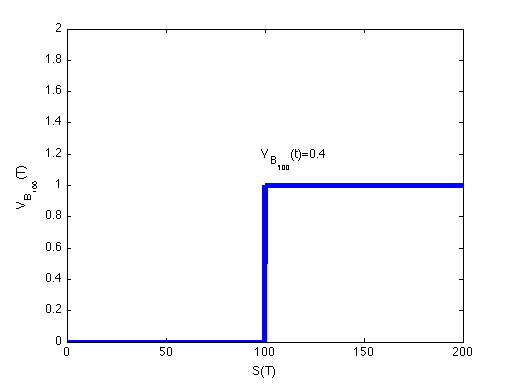
\includegraphics[width=3.5in]{pics/standardBinary}%
\captionof{figure}{$B_{100}$: A binary with strike $100$}\label{fig:standardBinary}%
\end{center}

% \begin{figure}[ht]
%\centering
 % 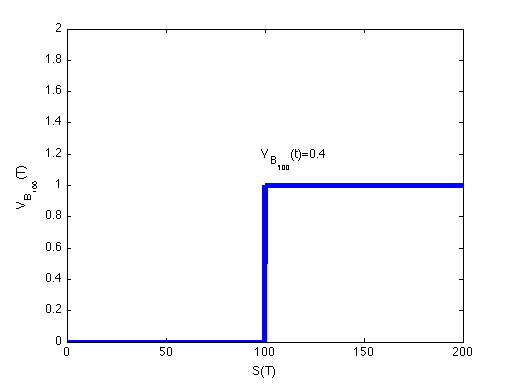
\includegraphics[width=4in] {pics/standardBinary}
%\caption{$B_{100}$: A binary with strike $100$}
%\label{fig:standardBinary}
%\end{figure}

Binaries are like little bricks. If you add enough bricks together you can make all sorts of shapes. The only restriction is that you can't make a shape that bends back on itself. So you can make the letter 'H', but not the letter 'G'. You can make a castle wall, but not a carriage wheel. 

Binaries contain information on the \textbf{risk neutral probability} of the event. This can be calculated for any strike where we have a binary price. If we have the price of binaries at all strikes we have the complete \textbf{risk neutral probability distribution} for the asset price at expiry. This is a nice thing to possess for three reasons:

\begin{enumerate}
\item It gives a complete market prediction of the probabilities of the asset being in any range of prices at expiry. This is a much richer prediction set than the forward price.
\item It can be used to price any other security with value dependent on the asset price at expiry.
\item It can be used to generate trades against any aspect of the distribution. For example, if you think the market predicted distribution is too 'fat tailed', you can construct a portfolio to bet against that.
\end{enumerate}

We'll explore these three characteristics in some detail.

\subsection{Making a binary}

%You can construct a binary from two call options. The construction process isn't perfect so constructed binaries are only \textit{approximately} equal to a theoretical binary. We'll assume that binaries can be constructed at the correct arbitrage free price. This comes from an assumption that an unlimited amount of options can be bought and sold at the unique `market price'.

To create a binary with strike $K$ buy a call option at $K_1$ slightly below $K$ and sell a call at $K_2$ slightly above $K$. The combined portfolio is in figure \ref{fig:buildingBinary}. As $K_1$ and $K_2$ get closer to $K$ the combination looks more and more like a binary that costs $V_{B_K} = V_{C_{K_2}}-V_{C_{K_1}}$ and pays $K_2-K_1$ if the price at expiry is above $K$. 

The example in figure \ref{fig:buildingBinary} uses $K=100$. A \textbf{collar} with $+C_{90}-C_{110}$ looks a little like the binary $B_{100}$; a collar with  $+C_{99}-C_{101}$ much more. The further we decrease the space between the the two call strikes the more the combination looks like a binary. 

  \begin{center}
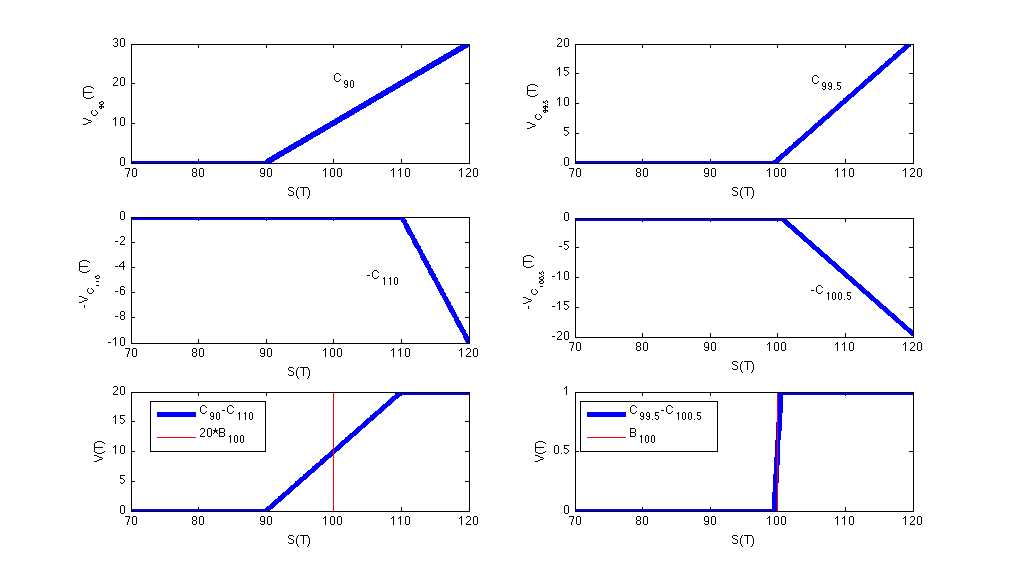
\includegraphics[width=5in]{pics/buildingBinary}%
\captionof{figure}{A binary is a very tight collar}\label{fig:buildingBinary}%
\end{center}

% \begin{figure}[ht]
%\centering
 % 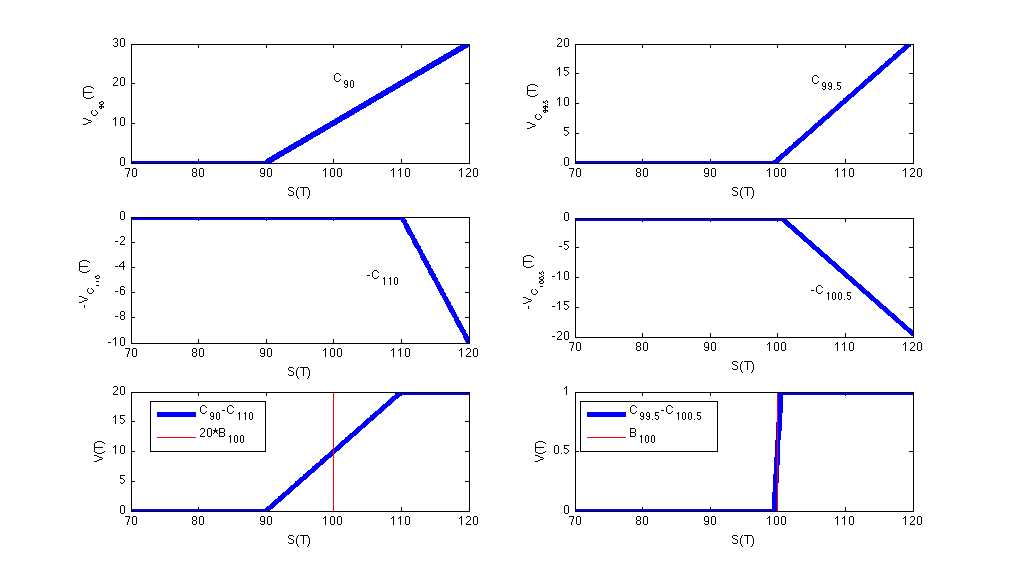
\includegraphics[width=4in] {pics/buildingBinary}
%\caption{A binary is a very tight collar}
%\label{fig:buildingBinary}
%\end{figure}

\subsection{A probability representation}

Someone offers you the following gamble:

\begin{itemize}
\item If it rains tomorrow they pay you \$2
\item If it doesn't rain tomorrow you pay them \$1
\item You pay \$0.2 to take the bet
\end{itemize}

Tthere is a value of the probability of rain tomorrow that makes this a fair gamble. Assuming that the risk free interest rate is zero (a dollar today is the same value as a dollar tomorrow) the probability makes the expected value of the bet equal to the cost:

\begin{eqnarray*}
P(\mbox{rain})*\$2 +P(\mbox{no rain})*-\$1 = \$0.2\\
\Rightarrow P(\mbox{rain}) = 0.4
\end{eqnarray*}

This value is called the \textbf{risk neutral probability} and it's the single most important thing to understand in finance. 

We can construct our binary bet in similar terms. The binary is the following gamble

\begin{itemize}
\item If the price of the asset at $T$ is above $K$ you get $K_2-K_1$
\item If the price of the asset at $T$ is below $K$ you get nothing
\item You pay $V_{B_K} = V_{C_{K_2}}-V_{C_{K_1}}$ to take the bet
\end{itemize}

The probability that makes this bet fair satisfies the following equation:

\begin{eqnarray*}
P(S(T)\geq K)*(K_2-K_1) + (1-P(S(T) \geq K))*0 =  \frac{1}{V_{Z_T}}\left(V_{C_{K_2}}-V_{C_{K_1}}\right)\\
\Rightarrow P(S(T)>K) = \frac{1}{V_{Z_T}}\frac{V_{C_{K_2}}-V_{C_{K_1}}}{K_2-K_1}
\end{eqnarray*}

The reciprocal of the zero coupon bond $Z_T$ is included to discount the value of the current cost of the options to the expiry.

If you're into calculus you can see that this is actually the first derivative of the value function with respect to the price

\begin{eqnarray*}
P(S(T) \geq K) &=\frac{1}{V_{Z_T(t)}} \lim_{K_1\rightarrow K_2} \frac{V_{C_{K_2}}-V_{C_{K_1}}}{K_2-K_1}
 &= \frac{1}{V_{Z_T(t)}}\frac{\partial V_{C_K}}{\partial K}
 \end{eqnarray*}

If calculus isn't your thing don't worry about that. The important thing is the implication that if we have the price of options at sufficiently close strikes we can calculate the risk neutral probabilities. 

\subsection{Making any function with binaries}

\subsubsection{Binary building blocks}
Say we have a binary which pays $x$ if event $E$ happens at time $T$, $y$ if $E$ doesn't happen, and costs $z$. We can transform this to a standard binary that pays \$1 if the event happens and \$0 if the event doesn't happen. We'll illustrate with an example first and then look at the general form.

\textbf{Example transforming a binary to a standard binary:}\\

The first panel in figure \ref{fig:binaryTransform} is a binary that pays \$6 if $S(1) \geq 100$ and \$-4 if  $S(1)<100$. Let's say it costs \$0.2 and that the borrowing/lending rate us $r(1) = 0.05$ so $V_{Z_1} = 0.9512$.  

\begin{center}
\begin{tabular}{|c|ccc|}
\hline
 & Value if $S(1)<100$ & Value if $S(1)\geq 100$ & Cost\\
 \hline
$B^{-4,6}_{100}$ & $-4$ & $6$ & $0.2$\\
\hline 
\end{tabular}
\end{center}

We want to turn this into something that pays \$0 or \$1. 

First we want something that pays in a \$1 range. We buy $\frac{1}{10}$ of the $B^{-4,6}_{100}$. This makes a binary $B^{-4/10,6/10}_{100}$.


\begin{center}
\begin{tabular}{|c|ccc|}
\hline
 & Value if $S(1)<100$ & Value if $S(1)\geq 100$ & Cost\\
 \hline
$B^{-4,6}_{100}$ & $-4$ & $6$ & $0.2$\\
$B^{-0.4,0.6}_{100}$ & $\frac{1}{10}*-4 = -0.4$ & $\frac{1}{10}*6 = 0.6$ & $\frac{1}{10}*0.2 = 0.02$\\
\hline 
\end{tabular}
\end{center}

Next we need to get rid of the -0.4. For this we buy a bond that pays $0.4$ no matter what happens. Added to the $B^{-0.4,0.6}_{100}$ this makes our desired binary.

\begin{center}
\begin{tabular}{|c|ccc|}
\hline
 & Value if $S(1)<100$ & Value if $S(1)\geq 100$ & Cost\\
 \hline
$B^{-4,6}_{100}$ & $-4$ & $6$ & $0.2$\\
$Z_1$ & 1 & 1 & 0.9512\\
$B^{-0.4,0.6}_{100}$ & $-0.4$ & $0.6$ & $0.02$\\
$0.4*Z_1$ & $0.4$ & $0.4$ & $0.4V_{Z_1} = 0.3805$\\
$B^{-0.4,0.6}_{100}+0.4*Z_1 = B^{0,1}$ & $0$ & $1$ & $0.3805+0.02 = 0.4005$\\
\hline 
\end{tabular}
\end{center}

 \begin{center}
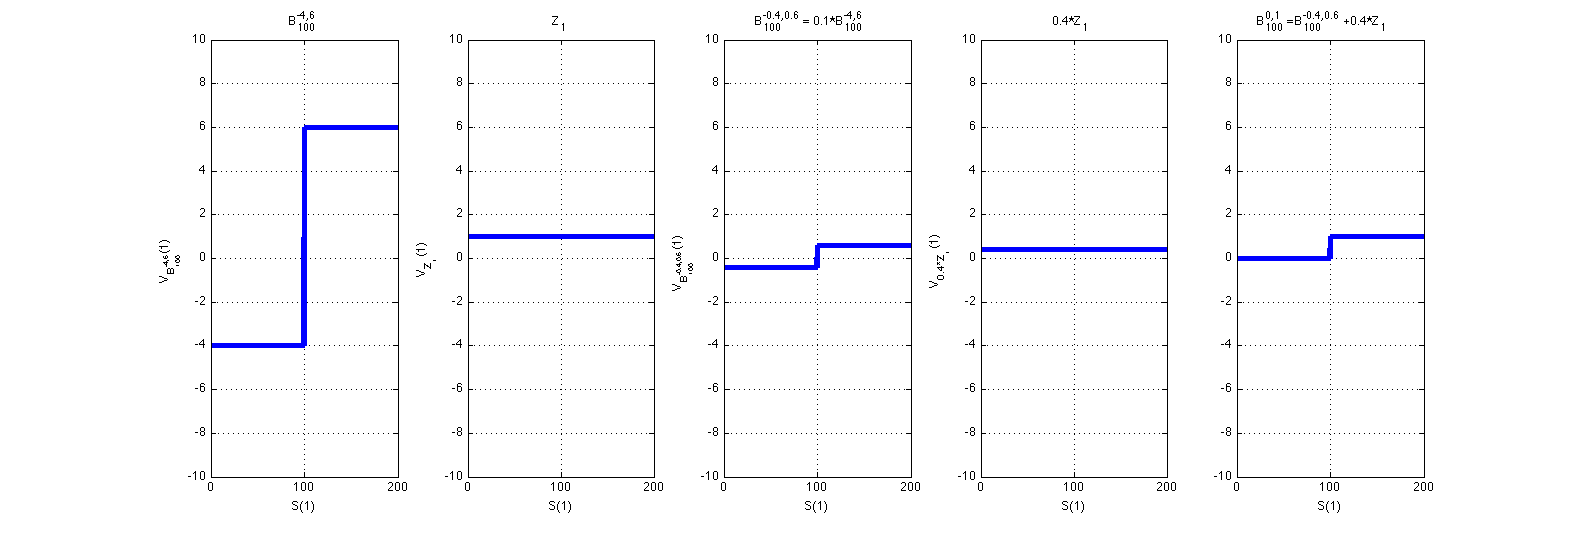
\includegraphics[width=6in]{pics/binaryTransform}%
\captionof{figure}{Creating a standard binary using a general binary and a bond}\label{fig:binaryTransform}%
\end{center}

% \begin{figure}[ht]
%\centering
 % 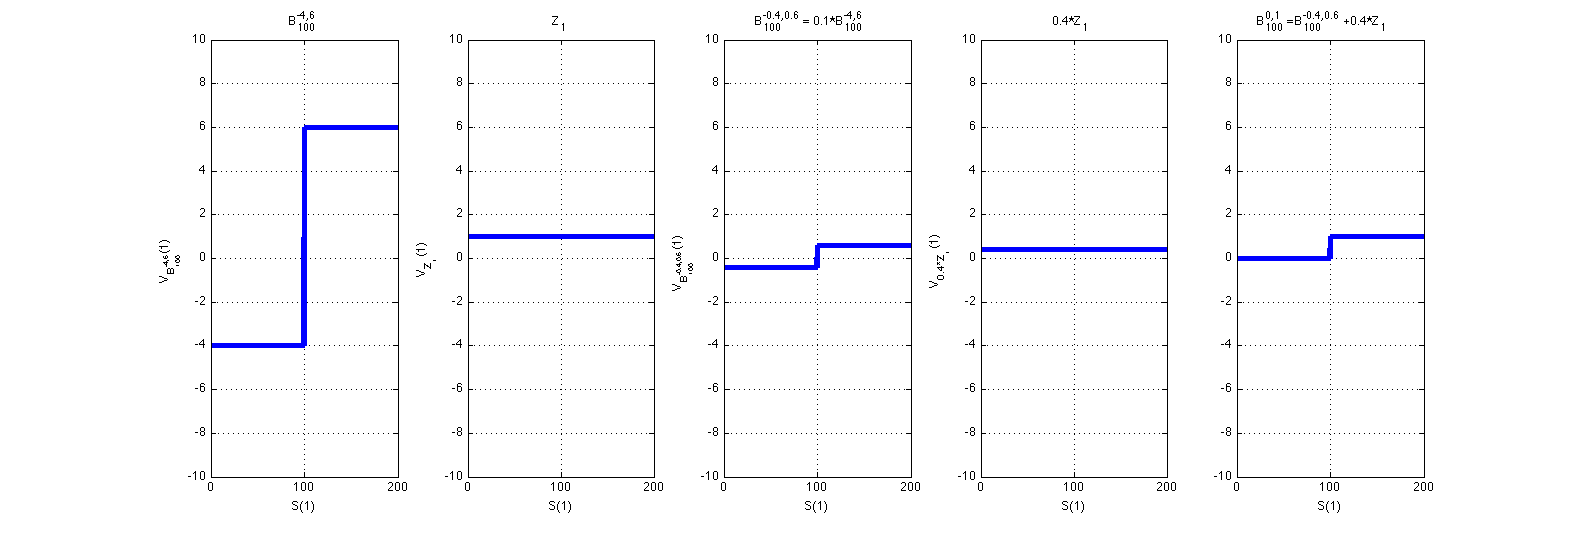
\includegraphics[width=6in] {pics/binaryTransform}
%\caption{Creating a standard binary using a general binary and a bond}
%\label{fig:binaryTransform}
%\end{figure}

The value of the binary is $V_{B_{100}} = 0.4005$. This also means the risk neutral probability is

\begin{eqnarray*}
 P(S(1)\geq100)*1+(1-P(S(1)\geq100))*0 = 0.4005\\
 \Rightarrow P(S(1)\geq 100) = 0.4005
 \end{eqnarray*}

We can use the standard binary without loss of generality because it can be transformed back to any scale we want. We get the same risk neutral probability if we calculate from the original binary.
 
 \textbf{General transformation of binary to standard binary}\\
 
 Back to the general form. The transformation process is:
 
 \begin{itemize}
 \item Start with binary that pays $x$ if event $E$ doesn't happen at time $T$, $y$ if $E$ does happen, and costs $z$. The binary is denoted $B^{x,y}_T$ and $V_{B^{x,y}_T} =z$
 \item Buy $\frac{1}{y-x}$ of the binary for $V_{B^{\frac{x}{y-x},\frac{y}{y-x}}_T} =\frac{z}{y-x}$
 \item Buy a bond that pays $\frac{-x}{y-x}$ at maturity. This costs $\frac{-x}{y-x}V_{Z_T}$
 \item The combination is equivalent to a binary $B^{  \frac{x}{y-x}- \frac{x}{y-x}  ,  \frac{y}{y-x}  -  \frac{x}{y-x}  }_T$ which is $B^{0,1}_T$
 \item The combination costs $\frac{z}{y-x}  -\frac{x}{y-x}V_{Z_T}$
 \end{itemize}

The risk neutral probability of the event is determined by solving

\[P(E)*1 + (1-P(E))*0 =  \frac{1}{V_{Z_T}} \left(\frac{z}{y-x}  -\frac{x}{y-x}V_{Z_T} \right) \]

It's a bit ugly like that but it makes sense in the example. If $x$ and $y$ are 0 and 1 this reduces to

\[P(E) = \frac{z}{V_{Z_T}}\]

\textbf{Building blocks}\\
With $+B_{K_1}-B_{K_2}$ we create a brick $|K_2-K_1|$ wide with height one (see figure \ref{fig:buildABlock}). We can buy more or less of each to change the height of the rectangle and vary strikes to change the width. So we can make any payoff that can be represented by stacks of arbitrary rectangle shapes. 

 \begin{center}
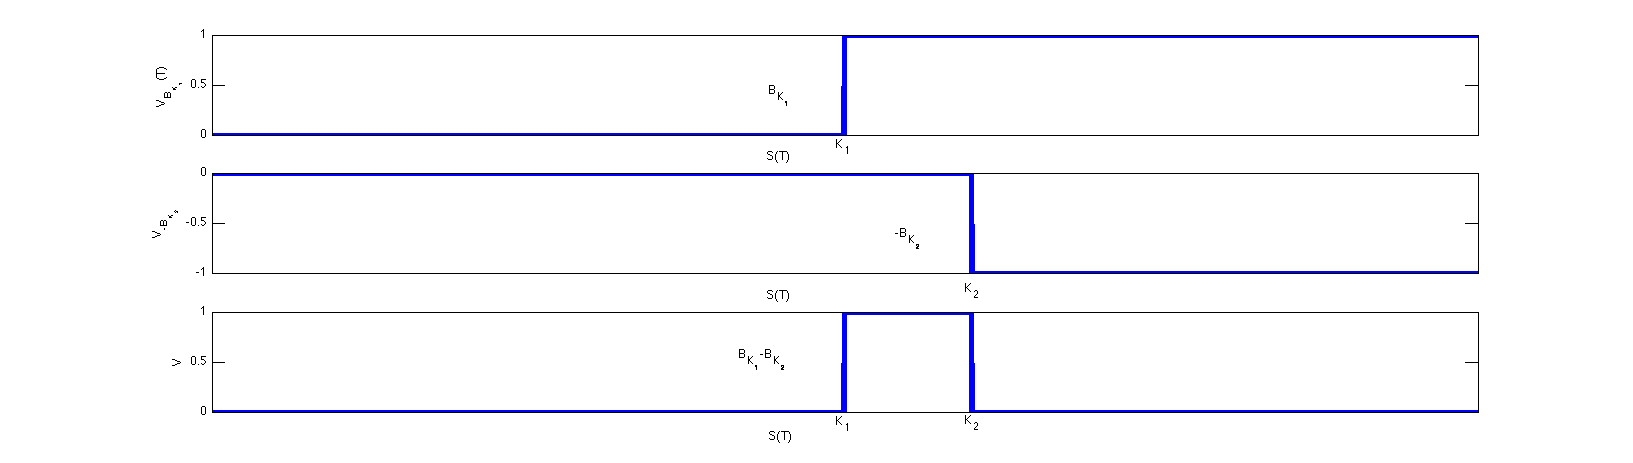
\includegraphics[width=6in]{pics/buildABlock}%
\captionof{figure}{Creating a block from two binaries}\label{fig:buildABlock}%
\end{center}

% \begin{figure}[ht]
%\centering
 % 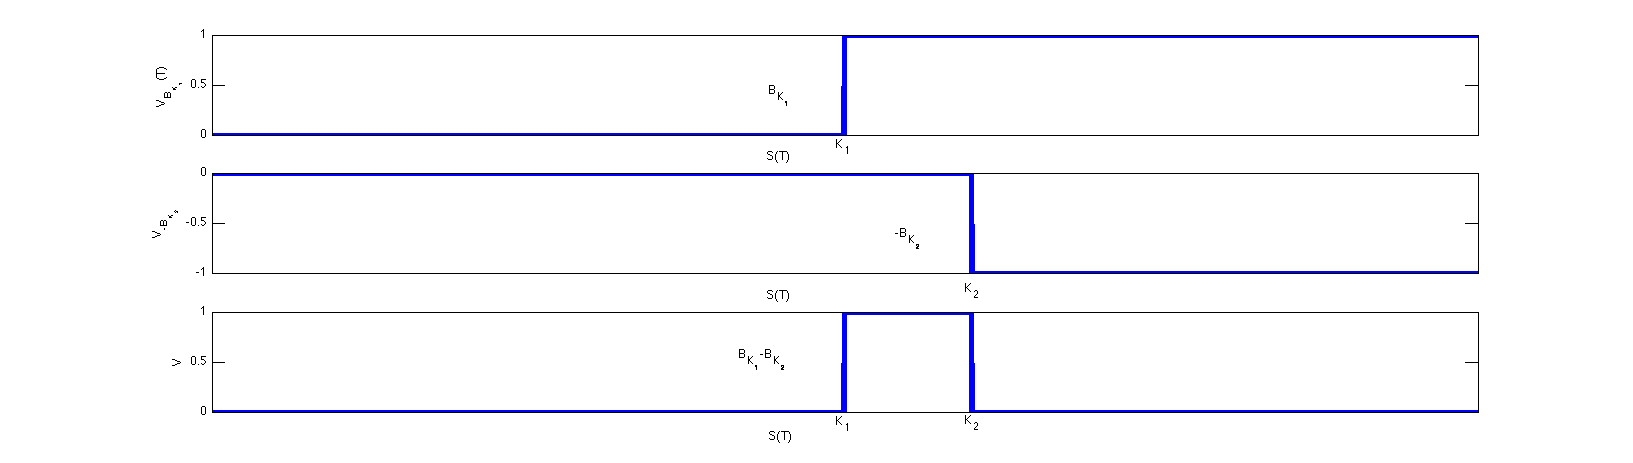
\includegraphics[width=6in] {pics/buildABlock}
%\caption{Creating a block from two binaries}
%\label{fig:buildABlock}
%\end{figure}

Say we wanted to make the letter "L" in the payoff diagram. We could do this with $+B_{1} - 0.8*B_{2}  -0.2*B_{4}$. (see figure \ref{fig:letterL}). In fact by this technique we can make any shape that is a function of the final asset value $S(T)$. There is a famous theorem that shows this precisely but it's quite intuitive if you imagine any function consisting of lots of little blocks.

 \begin{center}
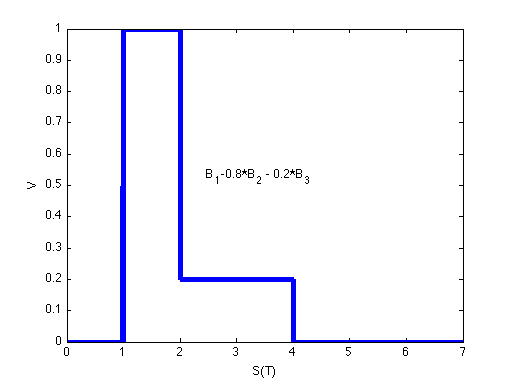
\includegraphics[width=4in]{pics/letterL}%
\captionof{figure}{The letter 'L' spelt with binaries}\label{fig:letterL}%
\end{center}

% \begin{figure}[ht]
%\centering
 % 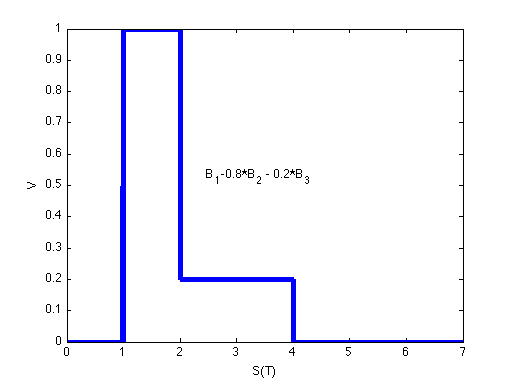
\includegraphics[width=3in] {pics/letterL}
%\caption{The letter 'L' spelt with binaries}
%\label{fig:letterL}
%\end{figure}

\subsection{Trading probabilities with binaries}

A single binary is a bet on its risk neutral probability. Combinations of binaries are bets on combinations of probabilities. With enough binaries we can bet on the entire distribution.  

For this section we'll distinguish between the \textbf{risk neutral probability} $P^Q$ and a \textbf{subjective probability} $P^S$. The subjective probability is our belief; if the subjective probability is different to the risk neutral probability we can construct a trade with a positive \textbf{expected value}. 

To keep things relatively simple we'll assume that the risk free rate is zero so that the price of the binaries can be taken directly as a probability.

\subsubsection{Trading a simple probability}

A standard binary that pays \$0 or \$1 will price on interval $(0,1)$. The price can be interpreted as the risk neutral probability of the asset price being above the strike at expiry. 

The expected value under the risk neutral distribution is zero by definition:

\begin{eqnarray*}
E^Q(V_{B^{0,1}_{KT}}(T)) = P^Q(S(T)<K)*0 + P^Q(S(T)\geq K)*1-\frac{V_{B_{K,T}^{0,1}}}{V_{Z_T}} = 0\\
\end{eqnarray*}

However the expected value under the subjective probability $P^S$ may be nonzero in which case there is a profitable (in expectation) trade:

\begin{eqnarray*}
E^S(V_{B^{0,1}_{KT}}(T)) = P^S(S(T)<K)*0 + P^S(S(T)\geq K)*1-\frac{V_{B_T^{0,1}}}{V_{Z_T}} \neq 0\\
 \Rightarrow \mbox{Buy or sell the binary} 
\end{eqnarray*}

You could be right and still lose money, but if you kept on being right and made enough similar trades you'd come out ahead. In figure \ref{fig:singleProb} the risk neutral probability is 0.4 but we believe the probability is actually 0.3. In this case we can sell the binary $B_{100}$.

 \begin{center}
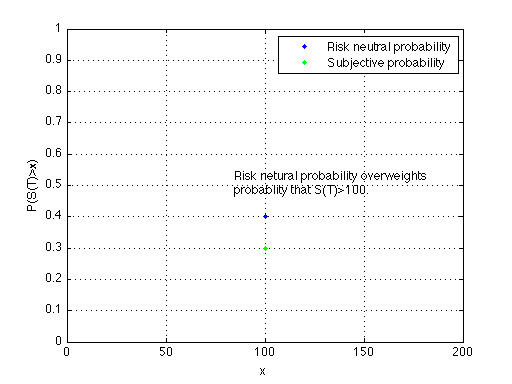
\includegraphics[width=4in]{pics/singleProb}%
\captionof{figure}{Risk neutral probability overestimates probability that price exceeds 100. }\label{fig:singleProb}%
\end{center}

% \begin{figure}[ht]
%\centering
 % 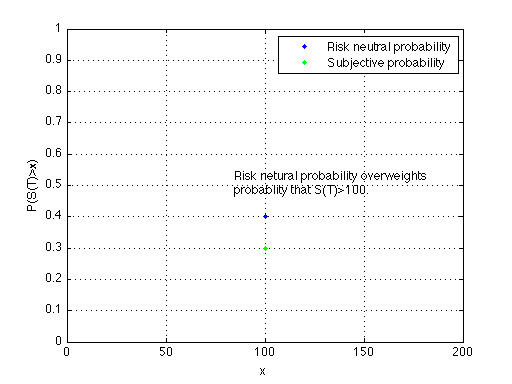
\includegraphics[width=3in] {pics/singleProb}
%\caption{Risk neutral probability overestimates probability that price exceeds 100. }
%\label{fig:singleProb}
%\end{figure}


\subsubsection{Trading a probability range}

We can trade a range of probabilities in a similar way. Let's say the binary $B_{100}$ costs 0.5 and the binary $B_{110}$ costs 0.2. We can interpret both the prices as risk neutral probabilities and the difference between the prices as the risk neutral probability of the range. The risk neutral probability of the price being above 100 is 50\%; the risk neutral probability of the price being above 110 is 20\%. Therefore the risk neutral probability of the price ending up between 100 and 110 is 0.5-0.2 = 0.3 = 30\%. 


(Note that the binary prices are equal to probabilities only if the risk free rate is zero so $V_{Z_T}=1$. We're assuming this to keep things simple.)

\begin{eqnarray*}
V_{B_{100}} = P(S(T)>100) =0.5\\
V_{B_{110}} = P(S(T)>110) = 0.2\\
\Rightarrow P(100<S(T)<110) = P(S(T)<110) - P(S(T)<100) = 0.3 
\end{eqnarray*}

Suppose that we have no strong views about the probability of the price \textbf{exceeding} 100 or 110, but a very strong view that the probability of the \textit{range} is 0.2. To trade the range rather than the individual probabilities we trade $-B_{100}+B_{110}$. This portfolio makes -\$1 if the price is in the range and \$0 if the price is outside the range. The portfolio costs -0.5+0.2 = -0.3 (so we get paid \$0.3 up front).  If the true probability is 0.2 the expected value of the trade is 

\[\underbrace{P^S(100<S(T)<110)}_{\mbox{probability of range}}*\underbrace{(-\$1)}_{\mbox{payoff in range}}- \underbrace{(-0.3)}_{\mbox{cost}} = \underbrace{0.1}_{\mbox{expected value}} \]

 \begin{center}
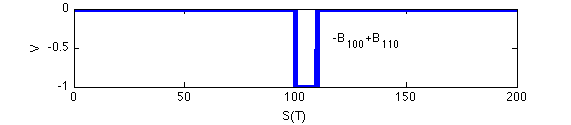
\includegraphics[width=6in]{pics/soldBinary}%
\captionof{figure}{$-B_{100}+B_{110}$ bets that the probability between these points is smaller than the risk neutral value}\label{fig: soldBinary}%
\end{center}

%\begin{figure}[ht]
%\centering
 % 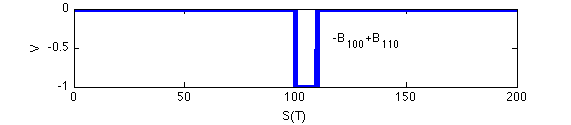
\includegraphics[width=3in] {pics/soldBinary}
%\caption{$-B_{100}+B_{110}$ bets that the probability between these points is smaller than the risk neutral value}
%\label{fig: soldBinary}
%\end{figure}

Our belief that the range probability is 0.2 doesn't pin down the probabilities of each side of the range. We could have $P(S(T)>100) = 0.2$ and $P(S(T)>100) = 0$ or $P(S(T)>100) = 1$ and $P(S(T)>100) = 0.8$ to give the same probability for the range. In figure \ref{fig:probRange} we have the risk neutral probabilities from $B_{100}$ and $B_{110}$ and nine possible combinations of subjective probabilities that give the probability of the range being 20\%. For the purposes of the trade the composition of probabilities doesn't matter; all that matters the the difference between the two is 20\%.  

 \begin{center}
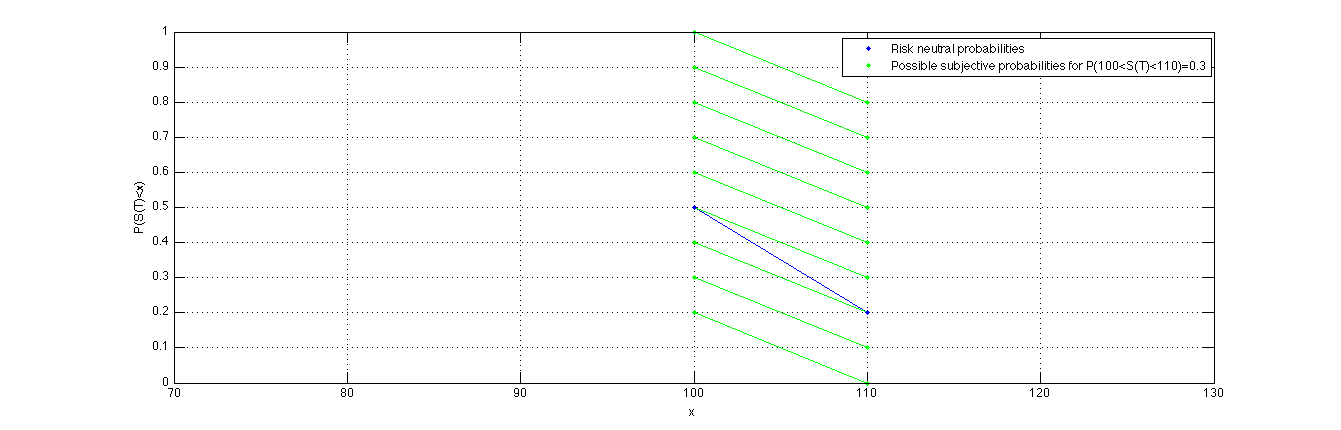
\includegraphics[width=6in]{pics/probRange}%
\captionof{figure}{Risk neutral probability overestimates probability that the price will be between 100 and 110 at expiry}\label{fig:probRange}%
\end{center}

%\begin{figure}[ht]
%\centering
 % 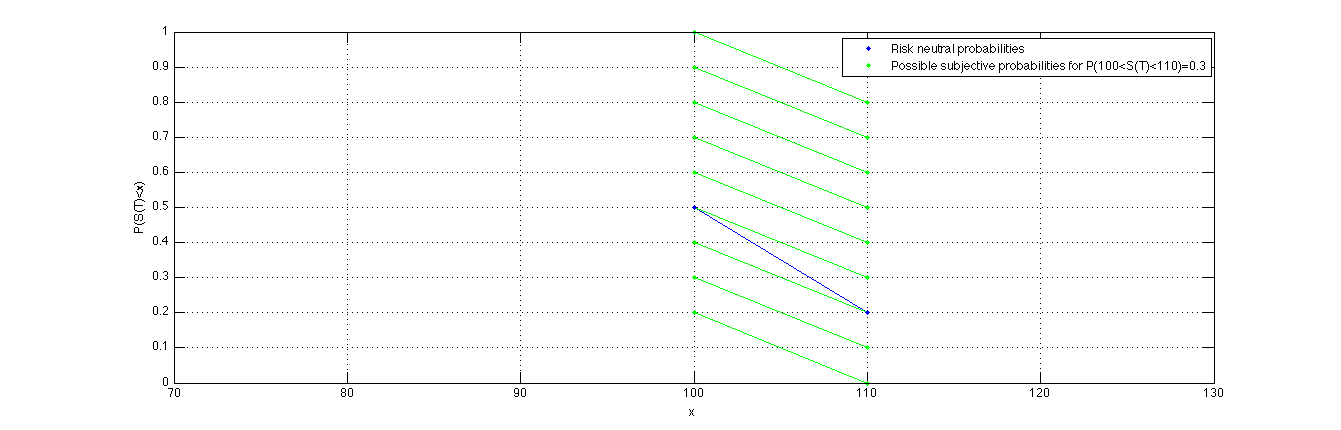
\includegraphics[width=3in] {pics/probRange}
%\caption{Risk neutral probability overestimates probability that the price will be between 100 and 110 at expiry }
%\label{fig:probRange}
%\end{figure}

\subsubsection{Trading the whole probability distribution}

If we have options at every strike we can extract a complete \textbf{risk neutral probability distribution}. We might also have a complete \textbf{subjective probability distribution} based on some beliefs that we hold. 

Consider a possible situation figure \ref{fig:probDist} with the risk neutral distribution in red and the subjective distribution in blue. In this example the subjective distribution is more \textbf{fat tailed} than the risk neutral distribution\footnote{The risk neutral distribution is t-distributed, the subjective distribution is Gaussian.} To express this belief we buy binaries in the tails and sell binaries in the centre of the distribution. Or something like that.

 \begin{center}
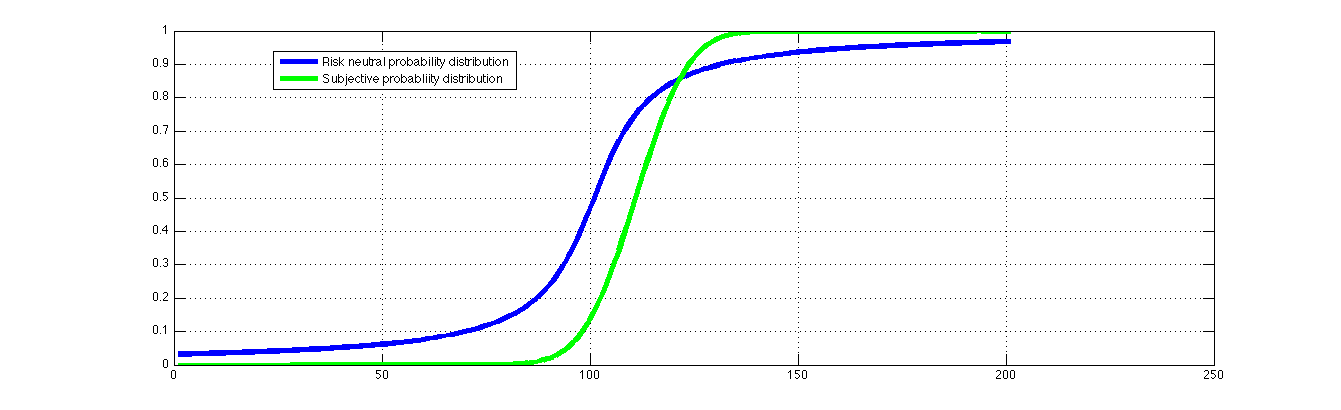
\includegraphics[width=6in]{pics/probDist}%
\captionof{figure}{Risk neutral probability overestimates probability in the tails}\label{fig:probDist}%
\end{center}

%\begin{figure}[ht]
%\centering
%  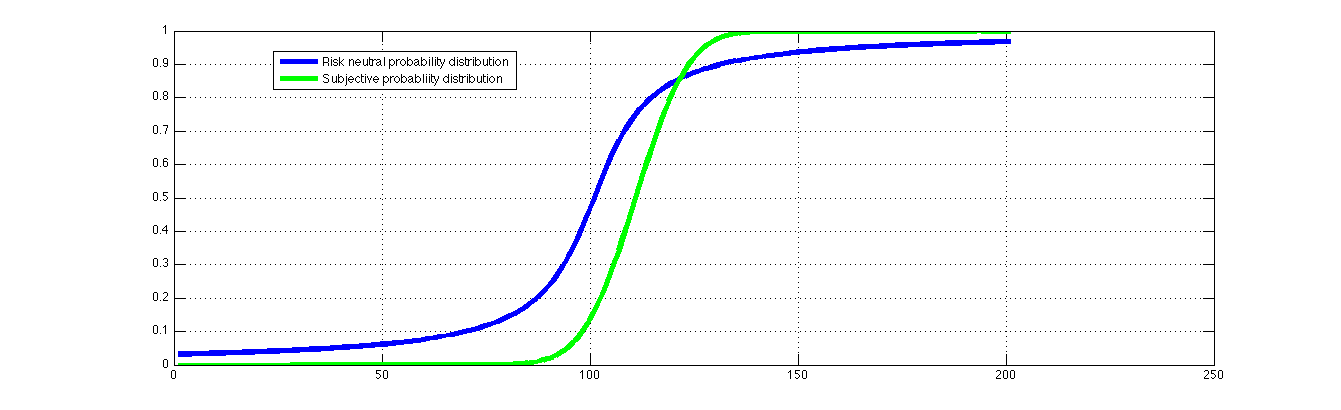
\includegraphics[width=5in] {pics/probDist}
%\caption{Risk neutral probability overestimates probability in the tails }
%\label{fig:probDist}
%\end{figure}

This is all a bit slip-shod. If we want to make more sophisticated combination trades to trade against certain parts of the risk natural distribution we need a little more theory. But the basic technique should now be plain. 


%\subsubsection{Trading the moments}

%Probability distributions are partly characterised by \textbf{moments} like the \textbf{mean}, \textbf{variance}, \textbf{skewness}, \textbf{kurtosis} and so forth. The risk neutral distribution has a value for each of these. It turns out we can construct portfolios that trade against each one of these moments. If we include dynamic hedges in the strategy we can construct \textbf{moment swaps} that pay the risk natural moment and receive the actual realised moment of the price distribution. This is a very powerful trading technique. We might be agnostic about the whether a price will go up or down but think the market is pricing the \textbf{variance} too high. We can construct a \textbf{variance swap} that receives the risk neutral variance and pays the \textbf{realised variance}. With such a portfolio we don't need to care about where the price ends up, only how volatile is the path it travails. 

%Many markets also price in significant skew. Interest rate options generally generate a \textbf{right skewed} risk neutral distribution. This means that the market expects volatility to be higher if interest rates are higher. If you disagree with this, or think the market overprices this effect, you can trade against it with a \textbf{skewness swap}.

%The exact development of these swaps is a little tricky so we postpone discussion to the advanced section on risk neutral distributions.


\section*{Questions}

\textbf{Question 1:} \\

(a) Turn a sold put at strike $K$ into a bought call at strike $K$\\
(b) Turn a sold call at strike $K$ into a bought put at strike $K$\\
(a) Turn a 25 delta risk reversal into a collar\\

\textbf{Question 2:}\\
Explain why the delta of a bought call minus one is the delta of a bought put.

\textbf{Question 3:}\\

Give greeks table for two options and create delta, gamma, delta-gamma, and vega hedge.


\textbf{Question 4:}\\

Say we have an asset $A$ with value 

\[V_A(t) = \log (S(t) ) \]

How many units of this asset are required to hedge an option with a gamma of 0.3?

\textbf{Question 5:}\\

A portly foreign stranger offers you a wager: if you can eat more bratwurst sausages than he you receive \$100, otherwise you must pay him \$5. What is the risk netural probability of you being the superior sausage eater?

\textbf{Question 6:}

The following prices for binaries prevail:

\begin{tabular}{|cc|}
\hline
Strike & Cost\\
\hline
1 & 0.7\\
5 & 0.4\\
10 & 0.1\\
\hline
\end{tabular}

Assuming that the risk free rate is zero:

\begin{itemize}
\item[(a)] What the the risk neutral probability that the asset will be worth more less than 1?
\item[(b)] What is the risk neutral probability that the asset will be worth between 1 and 10?
\item[(c )] You believe that the probability that that the asset will be worth between 1 and 5 is 40\%. What trade can you construct to exploit this belief? What is the expected value of the trade under your belief.
\end{itemize}

\textbf{Question 7:}

Redo question 6 if risk free rate is 10\% 

